\noindent Die Verfahren zur Datenanalyse multivariater Daten sind von dem Merkmalstyp des Eingangssignals und der Zielgr\"{o}{\ss}e abh\"{a}ngig. Korrelationsfunktionen und Regressionsfunktionen beschreiben die Abh\"{a}ngigkeit von Zielgr\"{o}{\ss}en als Funktion kontinuierlicher oder diskreter Eingangsgr\"{o}{\ss}en. Leider versagt diese mathematische Beschreibung bei ordinalen oder gruppierenden Eingangsgr\"{o}{\ss}en. Zum Beispiel l\"{a}sst sich die Frage, ob Spritzgussteile aus unterschiedlichen Formnestern A - D gleiche Abmessungen besitzen, nicht mit Regressionsfunktionen beantworten. Mithilfe eines Hypothesentests k\"{o}nnte bewertet werden, ob die Teile aus zwei Formnestern dieselbe Geometrie haben. Die vorgestellten Hypothesentests versagen jedoch bei mehr als zwei Gruppen. Die Varianzanalyse (ANOVA, \underbar{An}alysis \underbar{o}f \underbar{Va}riance) schlie{\ss}t diese L\"{u}cke und bewertet den Einfluss einer oder mehrerer ordinaler Eingangsgr\"{o}{\ss}en auf eine diskrete oder stetige Ausganggr\"{o}{\ss}e. \newline

\noindent Die Varianzanalyse wird mit einem Beispiel eingef\"{u}hrt. Bei der Fertigung von Bolzen muss sichergestellt werden, dass unterschiedliche Fertigungseinrichtungen zu beliebigen Zeitpunkten dieselbe Qualit\"{a}t liefern. Als kritisches Qualit\"{a}tsmerkmal der Bolzen wird der Bolzendurchmesser d gemessen, der normalen Fertigungsschwankungen unterliegt. Bei der Auswertung jeweils einer Stichprobe pro Fertigungscharge variiert der Mittelwert der Stichproben. Deshalb ist ein direkter Vergleich der Stichprobenmittelwerte von Charge zu Charge nicht aussagekr\"{a}ftig. Bild \ref{fig:EinfuehrungBolzendurchmesser1} verdeutlicht diesen Zusammenhang f\"{u}r vier Fertigungschargen 1 - 4.

\noindent 
\begin{figure}[H]
  \centerline{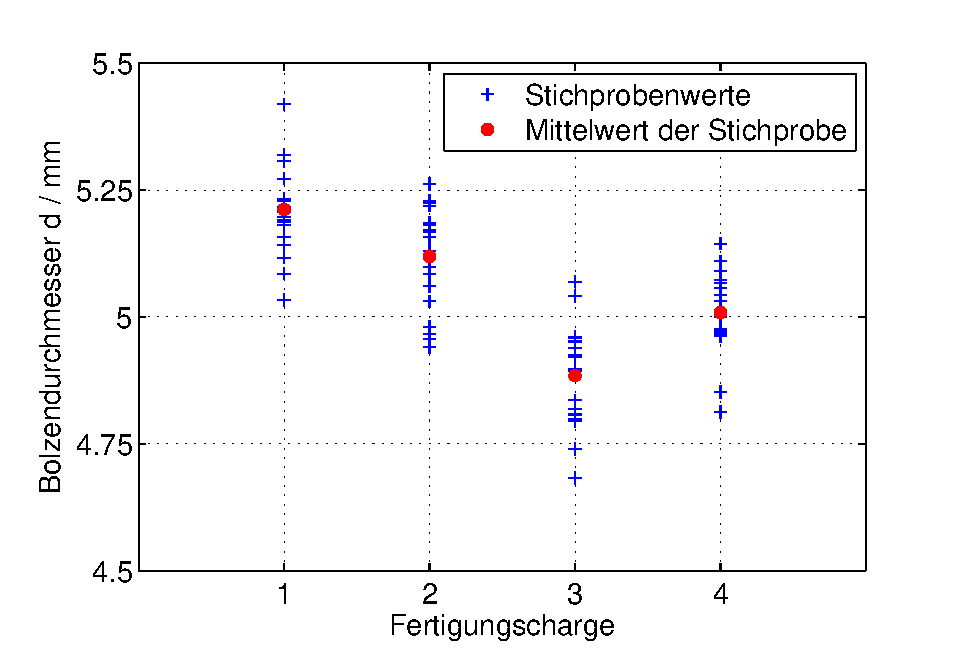
\includegraphics[width=0.5\textwidth]{Kapitel9/Bilder/image1}}
  \caption{Streuung der Stichprobenwerte bei der Fertigung von Bolzen und unterschiedlichen Fertigungschargen}
  \label{fig:EinfuehrungBolzendurchmesser1}
\end{figure}

\noindent Um zu entscheiden, ob die unterschiedlichen Chargen einen signifikanten Unterschied besitzen, muss versucht werden, den Einfluss der unterschiedlichen Chargen von der typischen Varianz des Prozesses zu trennen. Dies ist eine Aufgabe der einfaktoriellen Varianzanalyse. Die einfaktorielle Varianzanalyse pr\"{u}ft, ob zumindest eine Stichprobe signifikant von den anderen abweicht. \newline

\noindent Bei der Optimierung von Fertigungsprozessen werden teilweise auch ganz gezielt Fertigungsparameter ge\"{a}ndert. In diesem Fall wird der Einfluss unterschiedlicher Parameter\"{a}nderung auf die Zielgr\"{o}{\ss}e untersucht. Sollen M Einflussparameter gleichzeitig untersucht werden, m\"{u}ssen die von den Einflussfaktoren hervorgerufenen Varianzen und die normale Fertigungsvarianz voneinander getrennt werden. Dies ist eine Aufgabe der M-faktoriellen Varianzanalyse, die im Folgenden als ein- und zweifaktorielle Varianzanalyse hergeleitet und dann auf eine mehrfaktorielle Varianzanalyse verallgemeinert wird.

\clearpage

\noindent Diese Aufgabenstellungen werden bei der klassischen Varianzanalyse unter der Annahme bearbeitet, dass die Gruppen von Zahlen aus normalverteilten Grundgesamtheiten entstammen, die alle dieselbe Varianz $\sigma^{2}$ besitzen. Die Varianz $\sigma^{2}$ muss dabei nicht bekannt sein. Diese Annahme ist durch geeignete Hypothesentests vor Durchf\"{u}hren einer Varianzanalyse zu pr\"{u}fen. Sind die Annahmen nicht erf\"{u}llt, m\"{u}ssen parameterfreie Tests durchgef\"{u}hrt werden. 

\subsection{Einfaktorielle Varianzanalysen}

\noindent Bei einer einfaktoriellen Varianzanalyse wird der Einfluss einer ordinalen Eingangsgr\"{o}{\ss}e auf eine Zielgr\"{o}{\ss}e untersucht. Zur Darstellung der einfaktoriellen Varianzanalyse wird ein Fertigungsprozess betrachtet. In regelm\"{a}{\ss}igen Abst\"{a}nden wird auf Basis von Stichproben bewertet, ob sich die Zielwerte der vorliegenden Charge signifikant von den Werten der bisher gefertigten Chargen unterscheiden.

\subsubsection{Datenstruktur und Modellansatz der einfaktoriellen Varianzanalyse}

\noindent F\"{u}r die Bewertung werden J Fertigungslose untersucht, f\"{u}r jedes Fertigungslos sind die notwendigen Fertigungsparameter bekannt. Aus jedem Fertigungslos werden N Stichprobenwerte bestimmt.

\begin{table}[H]
\setlength{\arrayrulewidth}{.1em}
\caption{Nomenklatur zur Bezeichnung der Stichprobenwerte in Gruppen}
\setlength{\fboxsep}{0pt}%
\colorbox{lightgray}{%
\arrayrulecolor{white}%
\begin{tabular}{ wc{5.3cm} | wc{5.3cm} | wc{5.3cm} }
\hline\xrowht{10pt}

\fontfamily{phv}\selectfont{1.Fertigungslos} &
\fontfamily{phv}\selectfont{$\cdot$ j $\cdot$} &
\fontfamily{phv}\selectfont{J.Fertigungslos}  \\ \hline \xrowht{10pt}

\fontfamily{phv}\selectfont{$x_{11} \cdot x_{1n} \cdot x_{1N}$} &
\fontfamily{phv}\selectfont{$x_{j1} \cdot x_{jn} \cdot x_{jN}$} &
\fontfamily{phv}\selectfont{$x_{J1} \cdot x_{Jn} \cdot x_{JN}$}  \\ \hline 

\end{tabular}%
}
\label{tab:nineone}
\end{table}

\noindent Der erste Index j der Gr\"{o}{\ss}e $x_{jn}$ bezeichnet dabei die Nummer j des Fertigungsloses, das allgemein als Gruppe bezeichnet wird. Jede der J Gruppen besteht aus N Stichprobenwerten. Gepr\"{u}ft werden soll, ob hinsichtlich des Mittelwertes der Zielgr\"{o}{\ss}e bei den J Gruppen signifikante Unterschiede bestehen, die durch die unterschiedlichen Fertigungsparameter hervorgerufen wurden oder ob nur zufallsbedingte Streuungen vorliegen. Bestehen nur zufallsbedingte Unterschiede, ist es gleichg\"{u}ltig, mit welchen Fertigungsparametern die Bauteile gefertigt wurden. Weist ein Fertigungsparameter einen signifikanten Einfluss auf den Zielwert auf, kann er zum Beispiel zur Optimierung der Fertigungsausbeute oder zur Qualit\"{a}tsverbesserung verwendet werden.\newline

\noindent Es wird vorausgesetzt, dass die J Gruppen von Stichproben aus J normalverteilten Grundgesamtheiten stammen, die alle dieselbe Varianz $\sigma^{2}$ besitzen. Der einzelne Stichprobenwert $x_{jn}$ kann dann als Summe eines konstanten Mittelwertes µ, einer Abweichung zwischen den einzelnen Fertigungslosen $\alpha_{j}$ und einer zuf\"{a}lligen, normalverteilten Abweichung $\epsilon_{jn}$ dargestellt werden. Dabei wird davon ausgegangen, dass die Variablen $\mu$, $\alpha_{j}$ und $\epsilon_{jn}$ voneinander unabh\"{a}ngig sind.

\begin{equation}\label{eq:nineone}
x_{jn} =\mu +\alpha _{j} +\varepsilon _{jn}
\end{equation}

\noindent Damit kann die Varianzanalyse als Test der Hypothese aufgefasst werden, dass die J Gruppen aus derselben Grundgesamtheit mit dem Mittelwert $\mu$ stammen. Trifft diese Hypothese zu, besteht kein signifikanter Einfluss der Fertigungsparameter und die Abweichungen zwischen den einzelnen Fertigungslosen $\alpha$${}_{j}$ sind null.

\begin{equation}\label{eq:ninetwo}
\alpha _{1} =\alpha _{2} =\alpha _{3} =...=\alpha _{J} =0
\end{equation}

\noindent Die Gegenhypothese ist entsprechend, dass zumindest die Fertigungsparameter einer Stichprobe einen signifikanten Einfluss besitzen und damit gilt

\begin{equation}\label{eq:ninethree}
\alpha _{j} \ne 0
\end{equation}

\noindent F\"{u}r J = 2 Gruppen wird diese Aufgabe bei dem Hypothesentest zum Test auf gleichen Mittelwert bei unbekannter Varianz in Kapitel 6 behandelt. F\"{u}r J $\mathrm{>}$ 2 Gruppen wird die Aufgabe mit der Varianzanalyse gel\"{o}st. Hierbei wird davon ausgegangen, dass eine gro{\ss}e Streuung zwischen den Gruppen bei gleichzeitig geringer Streuung innerhalb der Gruppen auf eine gro{\ss}e Signifikanz des zu untersuchenden Prozessparameters hinweist. Damit wird der Hypothesentest abgelehnt, wenn die Streuung der Mittelwerte der Stichproben untereinander gr\"{o}{\ss}er ist als die Streuung innerhalb der Stichproben.

\noindent In dem Modellansatz aus Gleichung \eqref{eq:nineone} wird ein einzelner Stichprobenwert als Summe eines konstanten Mittelwertes µ, einer Abweichung zwischen den einzelnen Fertigungslosen $\alpha_{j}$ und einer zuf\"{a}lligen, normalverteilten Abweichung $\epsilon_{jn}$ dargestellt. Beide Gr\"{o}{\ss}en sind definitionsgem\"{a}{\ss} voneinander unabh\"{a}ngig. Aus Abschnitt 8.4.1 ist bekannt, dass die Varianz der Summe von unabh\"{a}ngigen Zufallsgr\"{o}{\ss}en als Summe der einzelnen Varianzen berechnet wird. Damit ergibt sich direkt aus dem Ansatz in Gleichung \eqref{eq:nineone} der Modellansatz der Varianzen aus den Stichprobenwerten der J Fertigungslose zu

\begin{equation}\label{eq:ninefour}
s_{x}^{2} =s_{\mu }^{2} +s_{\alpha }^{2} +s_{\varepsilon }^{2} =s_{\alpha }^{2} +s_{\varepsilon }^{2}
\end{equation}

\noindent Ziel des folgenden Abschnitts ist es, diese Varianzen herzuleiten.

\subsubsection{Berechnung der einzelnen Varianzen \"{u}ber die standardisierten Quadratsummen}

\noindent Mathematisch gesehen beruht die Berechnung der einzelnen Varianzen auf der Berechnung von Quadratsummen, die mit ihrer entsprechenden Anzahl von Freiheitsgraden normiert werden. Sie werden auch als standardisierte Quadratsummen bezeichnet. Bei der einfaktoriellen Varianzanalyse sind dies die standardisierten Quadratsummen M und M.\newline

\noindent Die Quadratsumme $q_{x}$, die die Abweichungen aller Stichprobenwerte von dem Gesamtmittelwert $\overline{x}$ beschreibt

\begin{equation}\label{eq:ninefive}
q_{x} =\sum _{j=1}^{J}\sum _{n=1}^{N}(x_{jn} -\bar{x})^{2}
\end{equation}

\noindent kann in Anteile zerlegt, die der entsprechenden Variationsursache entsprechen.

\begin{equation}\label{eq:ninesix}
\begin{split}
q_{x} & = \sum _{j=1}^{J}\sum _{n=1}^{N}(x_{jn} -\bar{x})^{2}   =\sum _{j=1}^{J}\sum _{n=1}^{N}(x_{jn} -\bar{x}_{j} +\bar{x}_{j} -\bar{x})^{2}\\
& = \sum _{j=1}^{J}\sum _{n=1}^{N}(x_{jn} -\bar{x}_{j})^{2} +2\cdot (x_{jn} -\bar{x}_{j})\cdot (\bar{x}_{j} -\bar{x}) + (\bar{x}_{j} -\bar{x}) ^{2}\\
& = N\cdot \sum _{j=1}^{J}(\bar{x}_{j} -\bar{x}) ^{2} + \sum _{n=1}^{N}\sum _{j=1}^{J}(x_{jn} -\bar{x}_{j})^{2} + 2\cdot \sum _{n=1}^{N}\sum _{j=1}^{J}(x_{jn} -\bar{x}_{j})\cdot (\bar{x}_{j} -\bar{x})
\end{split}
\end{equation}

\noindent Dabei berechnet sich der Mittelwert der j-ten Gruppe zu 

\begin{equation}\label{eq:nineseven}
\bar{x}_{j} =\dfrac{1}{N} \cdot \sum _{n=1}^{N}x_{jn}
\end{equation}

\noindent und der Gesamtmittelwert der Stichprobenwerte aller Gruppen zu

\begin{equation}\label{eq:nineeight}
\bar{x}=\dfrac{1}{J\cdot N} \cdot \sum _{j=1}^{J}\sum _{n=1}^{N}x_{jn}   =\dfrac{1}{J} \cdot \sum _{j=1}^{J}\bar{x}_{j}
\end{equation}

\noindent Der erste Summand in Gleichung \eqref{eq:ninesix}

\begin{equation}\label{eq:ninenine}
q_{\alpha } =N\cdot \sum _{j=1}^{J}\left(\bar{x}_{j} -\bar{x}\right)^{2}
\end{equation}

\noindent beschreibt die Streuung zwischen den Gruppen, indem er die Mittelwerte der Stichproben ${\overline{x}}_{j}$ von den unterschiedlichen Gruppen mit dem Gesamtmittelwert aller Stichproben $\overline{x}$ vergleicht. Die zweite Summe beschreibt die Streuung innerhalb der Gruppen

\begin{equation}\label{eq:nineten}
q_{\varepsilon } =\sum _{j=1}^{J}\sum _{n=1}^{N}(x_{jn} -\bar{x}_{j})^{2}
\end{equation}

\noindent Der dritte Summand kann umgerechnet werden zu 

\begin{equation}\label{eq:nineeleven}
\begin{split}
q_{0}  & = 2\cdot \sum _{j=1}^{J}\sum _{n=1}^{N}\left(x_{jn} -\bar{x}_{j} \right)\cdot \left(\bar{x}_{j} -\bar{x}\right)  =2\cdot \sum _{j=1}^{J}\sum _{n=1}^{N}(x_{jn} \cdot \bar{x}_{j} -x_{jn} \cdot \bar{x}-\bar{x}_{j} \cdot \bar{x}_{j} +\bar{x}_{j} \cdot \bar{x}) \\
& = 2\cdot \sum _{j=1}^{J}\sum_{n=1}^{N} x_{jn}\cdot \bar{x}_{j} -2\cdot N\cdot \sum _{j=1}^{J} \bar{x}_{j}\cdot \bar{x}-2\cdot\sum _{j=1}^{J}\sum_{n=1}^{N} x_{jn}\cdot \bar{x}_{j} + 2\cdot N\cdot \sum _{j=1}^{J} \bar{x}_{j}\cdot \bar{x} = 0
\end{split}
\end{equation}

\noindent Die Quadratsumme aus Gleichung \eqref{eq:ninesix} kann bei der einfaktoriellen Varianzanalyse damit in zwei Gruppen zerlegt werden, die die Streuung von Gruppe zu Gruppe beziehungsweise die Streuung innerhalb der Gruppen repr\"{a}sentiert.

\begin{equation}\label{eq:ninetwelve}
q_{x} =q_{\alpha } +q_{\varepsilon}
\end{equation}

\noindent Analog zu der Berechnung der Stichprobenvarianz in 3.3.2 m\"{u}ssen die berechneten Quadratsummen q und q auf ihre entsprechende Anzahl von Freiheitsgrade $\nu$ normiert werden, um die gesuchten Varianzen zu erhalten. Bei der Berechnung der Gesamtstreuung wird nur ein Mittelwert ben\"{o}tigt. Damit ergibt sich die standardisierte Quadratsumme durch Bezug auf die Anzahl der Stichproben J$.$N abz\"{u}glich eines Freiheitsgrades f\"{u}r einen festgelegten Parameter. Die Gesamtvarianz errechnet sich damit zu

\begin{equation}\label{eq:ninethirteen}
M_{x} =s_{x}^{2} =\dfrac{q_{x}}{\nu _{x}} =\dfrac{q_{\alpha} +q_{\varepsilon}}{J\cdot N-1}
\end{equation}

\noindent Die Berechnung der standardisierten Quadratsumme f\"{u}r den Einfluss der einzelnen J Gruppen ergibt sich analog durch Bezug auf die Anzahl der Gruppen J abz\"{u}glich eines Freiheitsgrades f\"{u}r den erforderlichen Mittelwert. 

\begin{equation}\label{eq:ninefourteen}
M_{\alpha} =s_{\alpha}^{2} =\dfrac{q_{\alpha}}{\nu _{\alpha}} =\dfrac{N\cdot \sum _{j=1}^{J}(\bar{x}_{j} -\bar{x})^{2}}{J-1}
\end{equation}

\noindent F\"{u}r den Einfluss der Reststreuung m\"{u}ssen J Mittelwerte bekannt sein, sodass J$.$N - J Freiheitsgrade vorliegen. 

\begin{equation}\label{eq:ninefifteen}
M_{\varepsilon} =s_{\varepsilon}^{2} =\dfrac{q_{\varepsilon}}{\nu _{\varepsilon}} =\dfrac{\sum _{j=1}^{J}\sum _{n=1}^{N}(x_{jn} -\bar{x}_{j})^{2}}{J\cdot N-J}
\end{equation}

\noindent Die berechneten Streuungskennwerte der Einzeleinfl\"{u}sse k\"{o}nnen damit auf ihre Signifikanz hin untersucht werden.

\subsubsection{Signifikanzbewertung der einzelnen Einfl\"{u}sse}

\noindent Die Bewertung der Varianzen der einzelnen Einfl\"{u}sse erfolgt \"{u}ber das Verh\"{a}ltnis der im Abschnitt 9.1.2 berechneten Varianzen. Dabei wird das Verh\"{a}ltnis der Streuung zwischen den Gruppen $s^{2}$ zu der Streuung innerhalb der Gruppen $s^{2}$ bewertet. Mit den Grundlagen aus 5.4.3 ist bekannt, dass die Zufallsvariable

\begin{equation}\label{eq:ninesixteen}
v_{0} =\dfrac{s_{\alpha}^{2}}{s_{\varepsilon }^{2}} =\dfrac{\dfrac{q_{\alpha}}{J-1}}{\dfrac{q_{\varepsilon}}{J\cdot (N-1)}}
\end{equation}

\noindent eine F-Verteilung mit den Freiheitsgraden $(J - 1, J\cdot (N - 1))$ aufweist. Liegt ein signifikanter Einfluss vor, wird die Varianz s² gro{\ss} und der Quotient $v_{0}$ steigt an. Ist der Einfluss nicht signifikant, wird der Quotient $v_{0}$ klein sein. Die Entscheidung auf Signifikanz beruht deshalb auf einen Vergleich des Quotienten der Varianzen $v_{0}$ mit einer Grenze c, die sich aus der F-Verteilung mit $(J - 1, J\cdot (N - 1))$ Freiheitsgraden und dem Signifikanzniveau $\alpha$ ergibt. 

\begin{equation}\label{eq:nineseventeen}
P(v\le c)=\gamma =1-\alpha
\end{equation}

\noindent Damit ergibt sich, dass im Fall v$v_{0}$ $\leq$ c die Hypothese der gleichen Mittelwerte $\alpha_{1} = \alpha_{2} = \dots = \alpha_{J} = 0$ angenommen wird, ist $v_{0} > c$ wird die Hypothese verworfen. Muss die Nullhypothese verworfen werden, kann auf Basis der vorliegenden Stichprobenwerte davon ausgegangen werden, dass die Gruppen einen signifikanten Unterschied besitzen. \newline

\noindent Alternativ kann der p-Wert, der zu der Variable $v_{0}$ geh\"{o}rt, mit dem Signifikanzniveau $\alpha = 1 - \gamma$ verglichen werden. Bild \ref{fig:FVerteilungSignifikanz} veranschaulicht den p-Wert bei der einfaktoriellen Varianzanalyse grafisch.

\noindent 
\begin{figure}[H]
  \centerline{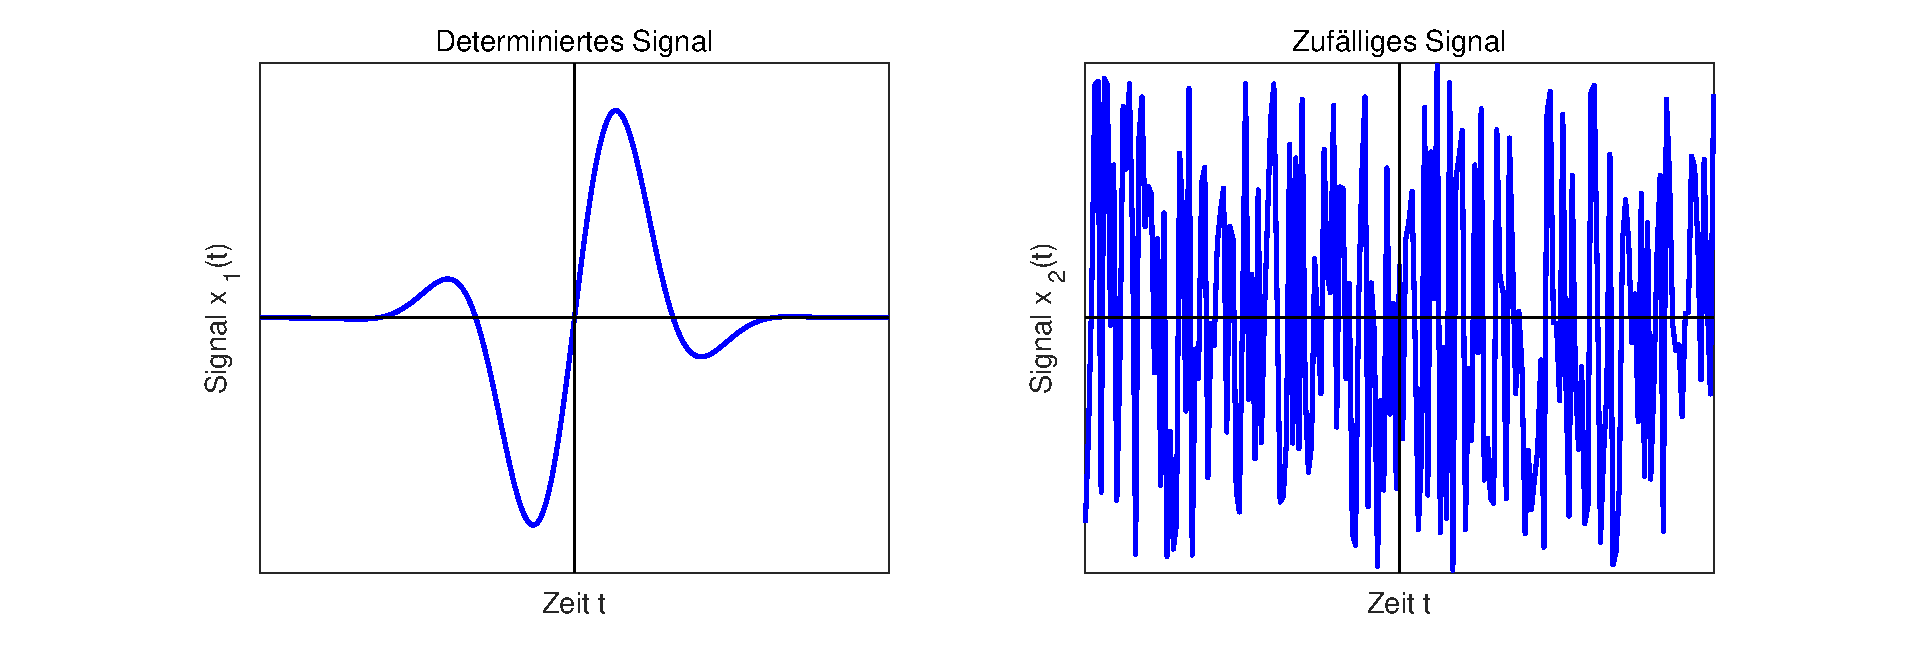
\includegraphics[width=0.5\textwidth]{Kapitel9/Bilder/image2}}
  \caption{p-Wert bei der einfaktoriellen Varianzanalyse}
  \label{fig:FVerteilungSignifikanz}
\end{figure}

\noindent Liegt der p-Wert oberhalb der Grenze $\alpha$, kann die Hypothese der gleichen Mittelwerte nicht verworfen werden. Der entsprechende Einflussfaktor w\"{a}re entsprechend nicht signifikant.

\begin{equation}\label{eq:nineeighteen}
p=1-F(v_{0})=1-F\left(\dfrac{s_{\alpha}^{2}}{s_{\varepsilon }^{2}} \right)
\end{equation}

\noindent Die Varianzanalyse wird typischerweise als ANOVA-Tabelle dargestellt. Dabei steht ANOVA f\"{u}r Analysis of Variance. Tabelle \ref{tab:ninetwo} zeigt den allgemeinen Aufbau einer einfaktoriellen ANOVA-Tabelle.

\begin{table}[H]
\setlength{\arrayrulewidth}{.1em}
\caption{Zusammenfassung der einfaktoriellen Varianzanalyse als ANOVA-Tabelle }
\setlength{\fboxsep}{0pt}%
\colorbox{lightgray}{%
\arrayrulecolor{white}%
\begin{tabular}{ wc{3.4cm} | wc{2cm} | wc{2cm} | wc{3.4cm} | wc{2cm} | wc{2cm} }
\hline\xrowht{10pt}

\fontfamily{phv}\selectfont{Streuungs-} &
\fontfamily{phv}\selectfont{Quadrat-} &
\fontfamily{phv}\selectfont{Freiheits-} &
\fontfamily{phv}\selectfont{Standardisierte} &
\fontfamily{phv}\selectfont{Wert der} &
\multirow{2}{*}{\fontfamily{phv}\selectfont{p-Wert}} \\ \xrowht{10pt}

\fontfamily{phv}\selectfont{quelle} &
\fontfamily{phv}\selectfont{summe} &
\fontfamily{phv}\selectfont{grade} &
\fontfamily{phv}\selectfont{Quadratsumme} &
\fontfamily{phv}\selectfont{Testvariable} &
\\\hline \xrowht{15pt}

\fontfamily{phv}\selectfont{Zwischen} &
\multirow{3}{*}{\fontfamily{phv}\selectfont{$q_{\alpha}$}} &
\multirow{3}{*}{\fontfamily{phv}\selectfont{$J-1$}} &
\multirow{3}{*}{\fontfamily{phv}\selectfont{$s_{\alpha}^{2} =\dfrac{q_{\alpha}}{J-1}$}} &
\multirow{6}{*}{\fontfamily{phv}\selectfont{$v_{0} =\dfrac{s_{\alpha}^{2}}{s_{\varepsilon}^{2}}$}} &
\multirow{6}{*}{\fontfamily{phv}\selectfont{$P(v>v_{0})$}} \\ \xrowht{15pt}

\fontfamily{phv}\selectfont{den Gruppen} &
&
&
&
&
\\\cline{1-4} \xrowht{15pt}

\fontfamily{phv}\selectfont{Innerhalb} &
\multirow{3}{*}{\fontfamily{phv}\selectfont{$q_{\epsilon}$}} &
\multirow{3}{*}{\fontfamily{phv}\selectfont{$J\cdot (N-1)$}} &
\multirow{3}{*}{\fontfamily{phv}\selectfont{$s_{\epsilon}^{2} =\dfrac{q_{\epsilon}}{J\cdot (N-1)}$}} &
&
\\ \xrowht{15pt}

\fontfamily{phv}\selectfont{der Gruppen} &
&
&
&
&
\\\hline \xrowht{15pt}

\fontfamily{phv}\selectfont{Gesamtstreuung} &
\fontfamily{phv}\selectfont{$q_{x}$} &
\fontfamily{phv}\selectfont{$J\cdot N-1$}&
&
&
\\\hline

\end{tabular}%
}
\label{tab:ninetwo}
\end{table}

\noindent Das Vorgehen zu diesem Test ist in Tabelle \ref{tab:ninethree} dargestellt.

\clearpage

\begin{table}[H]
\setlength{\arrayrulewidth}{.1em}
\caption{Test der Hypothese, dass die normalverteilten Grundgesamtheiten gleicher Varianz, aus denen J Gruppen stammen, alle denselben Mittelwert besitzen }
\setlength{\fboxsep}{0pt}%
\colorbox{lightgray}{%
\arrayrulecolor{white}%
\begin{tabular}{| wc{1cm} | wc{7.5cm} | wc{7.5cm}}
\xrowht{15pt}

\fontfamily{phv}\selectfont\textbf{Nr.} & 
\multicolumn{2}{c}{\fontfamily{phv}\selectfont\textbf{Prozessschritt}}\\ \hline \xrowht{20pt}

\fontfamily{phv}\selectfont{1} &
\multicolumn{2}{c}{\fontfamily{phv}\selectfont{Wahl eines Signifikanzniveaus $\alpha$}}\\ \hline \xrowht{10pt}

\multirow{4}{*}{\fontfamily{phv}\selectfont{2}} &
\multicolumn{2}{c}{\fontfamily{phv}\selectfont{Bestimmung des zugehörigen Parameters c aus der inversen F-Verteilung}} \\ \xrowht{10pt}
& \multicolumn{2}{c}{\fontfamily{phv}\selectfont{mit (J - 1, J$\cdot$N - J) Freiheitsgraden}}  \\\xrowht{25pt}
& \multicolumn{2}{c}{\fontfamily{phv}\selectfont{F(c) = 1 - $\alpha$}}  \\ \hline
\xrowht{20pt}

\multirow{4}{*}{\fontfamily{phv}\selectfont{3}} &
\multicolumn{2}{c}{\fontfamily{phv}\selectfont{Berechnung der J Mittelwerte der Gruppen und des Mittelwertes}} \\ \xrowht{10pt}
& \multicolumn{2}{c}{\fontfamily{phv}\selectfont{der gesamten Stichprobe}}  \\\xrowht{25pt}
& \multicolumn{2}{c}{\fontfamily{phv}\selectfont{$\bar{x}_{j} =\dfrac{1}{N} \cdot \sum _{n=1}^{N}x_{in} \qquad \qquad \qquad \qquad \qquad \qquad \bar{x}=\dfrac{1}{J\cdot N} \cdot \sum _{j=1}^{J}\sum _{n=1}^{N}x_{jn}=\dfrac{1}{J} \cdot \sum _{j=1}^{J}\bar{x}_{j}$}}  \\ \hline
\xrowht{20pt}

\multirow{6}{*}{\fontfamily{phv}\selectfont{4}} &
\multicolumn{2}{c}{\fontfamily{phv}\selectfont{Berechnung der der Varianz zwischen den Mittelwerten der Gruppe und}} \\ \xrowht{10pt}
& \multicolumn{2}{c}{\fontfamily{phv}\selectfont{des Mittelwertes der gesamten Stichprobe}}  \\\xrowht{30pt}
& \multicolumn{2}{c}{\fontfamily{phv}\selectfont{$s_{\alpha }^{2} =\dfrac{N\cdot \sum _{j=1}^{J}\left(\bar{x}_{j} -\bar{x}\right)^{2}  }{J-1} \qquad \qquad \qquad \qquad \qquad \qquad \qquad s_{\varepsilon }^{2} =\dfrac{q_{\varepsilon}}{\nu _{\varepsilon}} =\dfrac{\sum _{j=1}^{J}\sum _{n=1}^{N}\left(x_{jn} -\bar{x}_{j} \right)^{2}}{J\cdot N-J}$}}  \\ \hline
\xrowht{20pt}

\multirow{6}{*}{\fontfamily{phv}\selectfont{5}}  &
\multirow{2}{*}{\fontfamily{phv}\selectfont{Bestimmung des Annahmebereichs}} & \fontfamily{phv}\selectfont{Berechnung des p-Values mit der} \\
& & \fontfamily{phv}\selectfont{f-Verteilung} \\ \xrowht{40pt}
& \fontfamily{phv}\selectfont{$\dfrac{s_{\alpha }^{2} }{s_{\varepsilon }^{2} } <c$} & 
\fontfamily{phv}\selectfont{$p=1-F\left(\dfrac{s_{\alpha}^{2}}{s_{\varepsilon}^{2}} \right)$} \\ \hline\xrowht{15pt}

\multirow{4}{*}{\fontfamily{phv}\selectfont{6}}  &
\fontfamily{phv}\selectfont{F\"{u}r $s_{\alpha}^{2} / s_{\epsilon}^{2} < c$ wird die Hypothese} & 
\fontfamily{phv}\selectfont{F\"{u}r $p < 1 - \alpha$ wird die Hypothese} \\ \xrowht{15pt}
& \fontfamily{phv}\selectfont{angenommen, f\"{u}r $s_{\alpha}^{2} / s_{\epsilon}^{2} \geq c$ wird die} & \fontfamily{phv}\selectfont{angenommen, f\"{u}r p $ p \ge 1 - \alpha$ wird die } \\ \xrowht{15pt}
&  \fontfamily{phv}\selectfont{Hypothese verworfen} & \fontfamily{phv}\selectfont{Hypothese verworfen } \\ \hline

\end{tabular}%
}\bigskip
\label{tab:ninethree}
\end{table}

\noindent
\colorbox{lightgray}{%
\arrayrulecolor{white}%
\renewcommand\arraystretch{0.6}%
\begin{tabular}{ wl{16.5cm} }
{\fontfamily{phv}\selectfont
\noindent{Beispiel: Kondensatorfertigung}}
\end{tabular}%
}\medskip

\noindent Das Vorgehen wird anhand eines Beispiels verdeutlicht, in dem eine Kondensatorfertigung untersucht wird. Auf J = 3 Fertigungseinrichtungen mit gleichen Fertigungsparametern werden 47 nF - Kondensatoren gefertigt. Mithilfe einer einfaktoriellen Varianzanalyse soll festgestellt werden, ob die Fertigungsrichtung einen signifikanten Einfluss auf den Kapazit\"{a}tswert besitzt. Dazu werden je Fertigungseinrichtung N = 4 Kondensatoren untersucht, und es ergeben sich die in Tabelle \ref{tab:ninefour} gezeigten Messwerte.

\clearpage

\begin{table}[H]
\setlength{\arrayrulewidth}{.1em}
\caption{Stichprobe zur \"{U}berpr\"{u}fung der Fertigungseinrichtungen in der Kondensatorfertigung}
\setlength{\fboxsep}{0pt}%
\colorbox{lightgray}{%
\arrayrulecolor{white}%
\begin{tabular}{ wc{3.8cm} | wc{3.8cm} | wc{3.8cm} | wc{3.8cm} }
\hline\xrowht{15pt}

\fontfamily{phv}\selectfont{C / nF} &
\fontfamily{phv}\selectfont{Fertigungseinrichtung 1} &
\fontfamily{phv}\selectfont{Fertigungseinrichtung 2} &
\fontfamily{phv}\selectfont{Fertigungseinrichtung 3}  \\\hline \xrowht{10pt}

\multirow{4}{*}{\fontfamily{phv}\selectfont{Stichproben}} &
\fontfamily{phv}\selectfont{46.60} &
\fontfamily{phv}\selectfont{47.56} &
\fontfamily{phv}\selectfont{48.20}\\ \xrowht{10pt}

 &
\fontfamily{phv}\selectfont{48.20} &
\fontfamily{phv}\selectfont{47.24} &
\fontfamily{phv}\selectfont{47.56}\\ \xrowht{10pt}

 &
\fontfamily{phv}\selectfont{43.74} &
\fontfamily{phv}\selectfont{40.24} &
\fontfamily{phv}\selectfont{45.30}\\ \xrowht{10pt}

 &
\fontfamily{phv}\selectfont{46.60} &
\fontfamily{phv}\selectfont{46.60} &
\fontfamily{phv}\selectfont{47.88}\\ \hline \xrowht{10pt}

\fontfamily{phv}\selectfont{Gruppenmittelwert} &
\fontfamily{phv}\selectfont{46.29} &
\fontfamily{phv}\selectfont{45.41} &
\fontfamily{phv}\selectfont{47.24} \\\hline \xrowht{10pt}

\fontfamily{phv}\selectfont{Gesamtmittelwert} &
\multicolumn{3}{c}{\fontfamily{phv}\selectfont{46.31}} \\ \hline 

\end{tabular}%
}
\label{tab:ninefour}
\end{table}

\noindent Die Gruppenmittelwerte und der Mittelwert der gesamten Stichprobe sind bereits in die Tabelle eingetragen. Die Quadratsumme zwischen den Gruppen ist

\begin{equation}\label{eq:ninenineteen}
q_{\alpha} =N\cdot \sum _{j=1}^{J}(\bar{x}_{j} -\bar{x})^{2}  =4\cdot \left(0.02^{2} +0.9^{2} +0.93^{2} \right)=6.665
\end{equation}

\noindent Die Quadratsumme f\"{u}r die Varianz innerhalb der Gruppen ergibt sich aus

\begin{equation}\label{eq:ninetwenty}
q_{\varepsilon} =\sum _{j=1}^{J}\sum _{n=1}^{N}(x_{jn} -\bar{x}_{j})^{2} =(46.60-46.29)^{2} +...+(47.88-47.24)^{2} =51.656
\end{equation}

\noindent Damit berechnet sich die Gesamtquadratsumme zu

\begin{equation}\label{eq:ninetwentyone}
q_{x} =q_{\alpha} +q_{\varepsilon} =6.665+51.656=58.321
\end{equation}

\noindent Mit den berechneten Zahlenwerten l\"{a}sst sich der Quotient $v_{0}$ der Stichprobe bestimmen zu

\begin{equation}\label{eq:ninetwentytwo}
v_{0} =\dfrac{s_{\alpha}^{2}}{s_{\varepsilon}^{2}} =\dfrac{\dfrac{q_{\alpha}}{J-1}}{\dfrac{q_{\varepsilon}}{J\cdot (N-1)}} =\dfrac{\dfrac{6.665}{3-1}}{\dfrac{51.656}{3\cdot (4-1)}} =0.58062
\end{equation}

\noindent Mit dem Signifikanzniveau $\alpha = 0.05$, den Freiheitsgraden $(J - 1) = 2$ beziehungsweise $J \cdot (N - 1) = 9$ und der inversen F-Verteilung ergibt sich f\"{u}r 

\begin{equation}\label{eq:ninetwentythree}
F(c)=1-\alpha =0.95
\end{equation}

\noindent die kritische Grenze c = 4.26. Der Vergleich mit $v_{0}$ zeigt, dass $v_{0} < c $  ist. Die Hypothese, dass alle Mittelwerte gleich sind, wird deshalb best\"{a}tigt. Aufgrund der vorliegenden Stichprobe kann also angenommen werden, dass die unterschiedlichen Fertigungseinrichtungen keinen Einfluss auf den Kapazit\"{a}tswert haben. Der Kapazit\"{a}tswert schwankt nur zuf\"{a}llig zwischen den verschiedenen Fertigungseinrichtungen, der Unterschied der Fertigungseinrichtungen ist also nicht signifikant.\newline

\noindent Die Signifikanz des Einflusses der verschiedenen Fertigungseinrichtungen kann auch durch die Berechnung des p-Wertes gepr\"{u}ft werden. 

\begin{equation}\label{eq:ninetwentyfour}
p=1-F\left(\dfrac{s_{\alpha}^{2}}{s_{\varepsilon}^{2}} \right)=57.92\%
\end{equation}

\noindent Da die Wahrscheinlichkeit p mit 57.92\% \"{u}ber dem gew\"{a}hlten Signifikanzniveau von $\alpha= 5\% $ liegt, kann die Nullhypothese nicht verworfen werden. Dies stimmt mit der Einsch\"{a}tzung aus dem Vergleich der Gr\"{o}{\ss}e $v_{0}$ mit der berechneten Grenze c \"{u}berein.\newline

\noindent F\"{u}r das Beispiel ergibt sich mit den berechneten Daten die in Tabelle \ref{tab:ninefive} dargestellte ANOVA-Tabelle. Darin sind nochmals die wesentlichen Ergebnisse zusammengefasst, die f\"{u}r die Bewertung der Signifikanz des Einflusses der Fertigungseinrichtung ben\"{o}tigt werden.

\begin{table}[H]
\setlength{\arrayrulewidth}{.1em}
\caption{Bewertung der Fertigungseinrichtungen als ANOVA-Tabelle}
\setlength{\fboxsep}{0pt}%
\colorbox{lightgray}{%
\arrayrulecolor{white}%
\begin{tabular}{ wc{3.4cm} | wc{2cm} | wc{2cm} | wc{3.4cm} | wc{2cm} | wc{2cm} }
\hline\xrowht{10pt}

\fontfamily{phv}\selectfont{Streuungs-} &
\fontfamily{phv}\selectfont{Quadrat-} &
\fontfamily{phv}\selectfont{Freiheits-} &
\fontfamily{phv}\selectfont{Standardisierte} &
\fontfamily{phv}\selectfont{Wert der} &
\multirow{2}{*}{\fontfamily{phv}\selectfont{p-Wert}} \\ \xrowht{10pt}

\fontfamily{phv}\selectfont{quelle} &
\fontfamily{phv}\selectfont{summe} &
\fontfamily{phv}\selectfont{grade} &
\fontfamily{phv}\selectfont{Quadratsumme} &
\fontfamily{phv}\selectfont{Testvariable} &
\\\hline \xrowht{15pt}

\fontfamily{phv}\selectfont{Zwischen} &
\multirow{3}{*}{\fontfamily{phv}\selectfont{6.665}} &
\multirow{3}{*}{\fontfamily{phv}\selectfont{2}} &
\multirow{3}{*}{\fontfamily{phv}\selectfont{3.3325}} &
\multirow{6}{*}{\fontfamily{phv}\selectfont{0.58}} &
\multirow{6}{*}{\fontfamily{phv}\selectfont{0.5792}} \\ \xrowht{15pt}

\fontfamily{phv}\selectfont{den Gruppen} &
&
&
&
&
\\\cline{1-4} \xrowht{15pt}

\fontfamily{phv}\selectfont{Innerhalb} &
\multirow{3}{*}{\fontfamily{phv}\selectfont{51.6562}} &
\multirow{3}{*}{\fontfamily{phv}\selectfont{9}} &
\multirow{3}{*}{\fontfamily{phv}\selectfont{5.73958}} &
&
\\ \xrowht{15pt}

\fontfamily{phv}\selectfont{der Gruppen} &
&
&
&
&
\\\hline \xrowht{15pt}

\fontfamily{phv}\selectfont{Gesamtstreuung} &
\fontfamily{phv}\selectfont{58.3212} &
\fontfamily{phv}\selectfont{11} &
&
&
\\\hline

\end{tabular}%
}
\label{tab:ninefive}
\end{table}

\noindent Das Ergebnis l\"{a}sst sich auch mit einem Box-Plot grafisch plausibilisieren. Hierzu wird f\"{u}r jede Gruppe ein Box-Plot erzeugt und zum Vergleich nebeneinander dargestellt.

\noindent 
\begin{figure}[H]
  \centerline{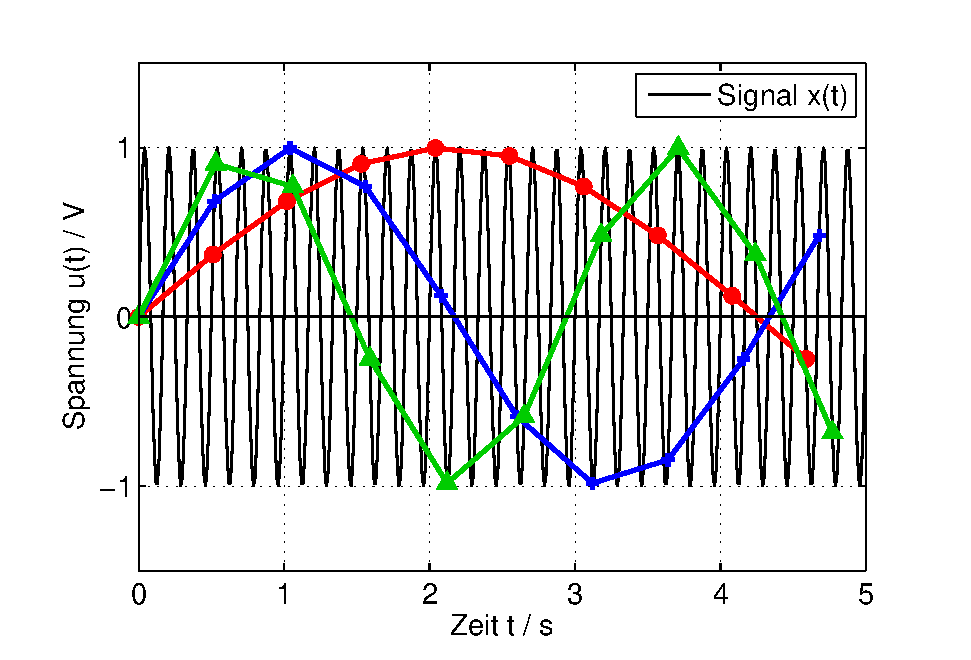
\includegraphics[width=0.5\textwidth]{Kapitel9/Bilder/image3}}
  \caption{Box-Plot f\"{u}r das Beispiel der Kondensatorfertigung}
  \label{fig:VarianzanalyseEinfachFertigung1}
\end{figure}

\noindent Der Box-Plot in Bild \ref{fig:VarianzanalyseEinfachFertigung1} zeigt, dass sich die Verteilungen \"{u}berlappen und deshalb hinsichtlich des Kapazit\"{a}tswertes kein signifikanter Unterschied zwischen den Gruppen besteht.\newline

\noindent Die Berechnung mit MATLAB ist in den folgenden Programmzeilen dargestellt.

\lstinputlisting[caption = {}]{Kapitel9/mat1.m}

\clearpage

\subsection{Mehrfaktorielle Varianzanalyse}

\noindent Bei der einfaktoriellen Varianzanalyse wird gezeigt, wie der Einfluss eines Parameters auf eine Zielgr\"{o}{\ss}e gepr\"{u}ft wird. Im Beispiel in Abschnitt 9.1 war dies der Einfluss der verschiedenen Fertigungseinrichtungen auf den Wert des produzierten Kondensators. In vielen F\"{a}llen ist die \"{U}berpr\"{u}fung eines Parameters nicht ausreichend, da eine Zielgr\"{o}{\ss}e oft von mehr als einer Einflussgr\"{o}{\ss}e abh\"{a}ngt. Zum Beispiel k\"{o}nnte der Kapazit\"{a}tswert von dem Zulieferer des Basismaterials, der Fertigungseinrichtung und dem Bediener der Fertigungseinrichtung abh\"{a}ngen. Um die Signifikanz dieser unterschiedlichen Einflussgr\"{o}{\ss}en zu untersuchen, kann eine mehrfaktorielle Varianzanalyse durchgef\"{u}hrt werden. Die Herleitung dazu wird wegen der vielen Indizes schnell un\"{u}bersichtlich. Aus diesem Grund beschr\"{a}nkt sich die Herleitung in diesem Abschnitt auf die zweifaktorielle Varianzanalyse. Die dabei erlangten Erkenntnisse k\"{o}nnen auf beliebig viele Dimensionen erweitert werden.

\subsubsection{Datenstruktur und Modellansatz der zweifaktoriellen Varianzanalyse}

\noindent Bei der zweifaktoriellen Varianzanalyse wird die Bewertung gegen\"{u}ber der einfaktoriellen Analyse um einen Einflussparameter $\beta$ und eine Wechselwirkung $\alpha\beta$ erweitert. Dazu muss zun\"{a}chst die Nomenklatur der Stichprobenbezeichnung gekl\"{a}rt werden. Die Stichprobenwerte k\"{o}nnen in Matrizenform dargestellt werden.
 
\begin{table}[H]
\setlength{\arrayrulewidth}{.1em}
\caption{Nomenklatur der Stichprobenindizes f\"{u}r die zweifaktorielle Varianzanalyse}
\setlength{\fboxsep}{0pt}%
\colorbox{lightgray}{%
\arrayrulecolor{white}%
\begin{tabular}{| wc{0.7cm}  wc{1cm} | wc{3.2cm} | wc{1.5cm} | wc{3.2cm} | wc{1.5cm} | wc{3.2cm} }
\xrowht{10pt}

& & 
\multicolumn{5}{c}{\fontfamily{phv}\selectfont{Einflussgröße $\beta$}}\\  \xrowht{10pt} 

& &
\fontfamily{phv}\selectfont{1} &
\fontfamily{phv}\selectfont{...} &
\fontfamily{phv}\selectfont{k} &
\fontfamily{phv}\selectfont{...} &
\fontfamily{phv}\selectfont{K} \\ \hline \xrowht{10pt} 

\multirow{7}{*}{\fontfamily{phv}\selectfont\rotatebox{90}{Einflussgröße $\alpha$}} &
\fontfamily{phv}\selectfont{1} & 
\fontfamily{phv}\selectfont{$x_{111} \dots x_{11n} \dots x_{11N}$} &
\fontfamily{phv}\selectfont{ } &
\fontfamily{phv}\selectfont{...} &
\fontfamily{phv}\selectfont{ } &
\fontfamily{phv}\selectfont{$x_{1K1} \dots x_{JKn} \dots x_{JKN}$}\\ \cline{2-7} \xrowht{10pt} 

& 
\fontfamily{phv}\selectfont{$\vdots$} & 
\fontfamily{phv}\selectfont{ } &
\fontfamily{phv}\selectfont{ } &
\fontfamily{phv}\selectfont{ } &
\fontfamily{phv}\selectfont{ } &
\fontfamily{phv}\selectfont{ }\\ \cline{2-7} \xrowht{10pt} 

& 
\fontfamily{phv}\selectfont{j} & 
\fontfamily{phv}\selectfont{$\vdots$} &
\fontfamily{phv}\selectfont{ } &
\fontfamily{phv}\selectfont{$x_{jk1} \dots x_{jkn} \dots x_{jkN}$} &
\fontfamily{phv}\selectfont{ } &
\fontfamily{phv}\selectfont{$\vdots$}\\ \cline{2-7} \xrowht{10pt} 

& 
\fontfamily{phv}\selectfont{$\vdots$} & 
\fontfamily{phv}\selectfont{ } &
\fontfamily{phv}\selectfont{ } &
\fontfamily{phv}\selectfont{ } &
\fontfamily{phv}\selectfont{ } &
\fontfamily{phv}\selectfont{ }\\ \cline{2-7} \xrowht{10pt}

& 
\fontfamily{phv}\selectfont{J} & 
\fontfamily{phv}\selectfont{$x_{J11} \dots x_{J1n} \dots x_{J1N}$} &
\fontfamily{phv}\selectfont{ } &
\fontfamily{phv}\selectfont{...} &
\fontfamily{phv}\selectfont{ } &
\fontfamily{phv}\selectfont{$x_{JK1} \dots x_{JKn} \dots x_{JKN}$}\\ \hline

\end{tabular}%
}\bigskip
\label{tab:ninesix}
\end{table}

\noindent Der Zeilenindex j l\"{a}uft von 1 bis J, der Spaltenindex k von 1 bis K. In jeder Gruppe befinden sich N Stichprobenwerte, die mit dem Index n bezeichnet werden. Damit ergibt sich die Bezeichnung f\"{u}r den einzelnen Stichprobenwert $x_{jkn}$.\newline

\noindent Der einzelne Stichprobenwert $x_{jkn}$ kann als Summe eines konstanten Mittelwertes µ, den systematischen Abweichungen $\alpha_{j}$ und $\beta_{k}$, der Wechselwirkung der beiden Gr\"{o}{\ss}en $\alpha\beta_{jk}$ sowie einer zuf\"{a}lligen, normalverteilten Abweichung $\epsilon_{jkn}$ dargestellt werden.

\begin{equation}\label{eq:ninetwentyfive}
x_{jkn} =\mu +\alpha _{j} +\beta _{k} +\alpha \beta _{jk} +\varepsilon _{jkn}   
\end{equation}

\noindent Die Analyse der Frage, ob bez\"{u}glich eines Faktors oder der Wechselwirkung ein signifikanter Einfluss vorliegt, entspricht wieder einem Hypothesentest. Zum Beispiel kann die Signifikanz des Faktors $\alpha_{j}$ untersucht werden. Besitzt der Faktor keine Signifikanz, ist f\"{u}r $\alpha_{j}$ ein Wert nahe null zu erwarten. Damit lautet die Nullhypothese:

\begin{equation}\label{eq:ninetwentysix}
\alpha _{1} =\alpha _{2} =\alpha _{3} =...=\alpha _{J} =0
\end{equation}

\noindent Die Gegenhypothese lautet, dass zumindest eine Stichprobe einen signifikanten Einfluss $\alpha_{j}$ besitzt, und es gilt:

\begin{equation}\label{eq:ninetwentyseven}
\alpha _{j} \ne 0
\end{equation}

\noindent Diese Form des Hypothesentests kann auf gleiche Weise auch f\"{u}r den Einflussfaktor $\beta$ und die Wechselwirkung $\alpha \beta$ angewendet werden. Wie bei der einfaktoriellen Varianzanalyse kann direkt aus dem Modellansatz aus Gleichung \eqref{eq:ninetwentyfive} der Modellansatz der Varianzen aus den Stichprobenwerten angegeben werden.

\begin{equation}\label{eq:ninetwentyeight}
s_{x}^{2} =s_{\alpha}^{2} +s_{\beta}^{2} +s_{\alpha \beta}^{2} +s_{\varepsilon}^{2}
\end{equation}

\noindent Die Bestimmung der Varianzen erfolgt analog zur einfaktoriellen Varianzanalyse \"{u}ber die Berechnung von Quadratsummen, die auf ihre Anzahl von Freiheitsgraden normiert werden.

\subsubsection{Berechnung der einzelnen Varianzen \"{u}ber die standardisierten Quadratsummen}

\noindent Wie bei der einfaktoriellen Varianzanalyse bildet auch im mehrdimensionalen Fall die Quadratsumme der Abweichungen der Stichprobenwerte vom Mittelwert die Grundlage der Berechnung. Die Quadratsumme

\begin{equation}\label{eq:ninetwentynine}
q_{x} =\sum _{j=1}^{J}\sum _{k=1}^{K}\sum _{n=1}^{N}(x_{jkn} -\bar{x})^{2}
\end{equation}

\noindent kann analog zur einfaktoriellen Varianzanalyse zerlegt werden in

\begin{equation}\label{eq:ninethirty}
\begin{split}
q_{x} & = \sum _{j=1}^{J}\sum _{k=1}^{K}\sum _{n=1}^{N}(\bar{x}_{j} -\bar{x})^{2}    +\sum _{j=1}^{J}\sum _{k=1}^{K}\sum _{n=1}^{N}(\bar{x}_{k} -\bar{x})^{2}
\end{split}
\end{equation}

\noindent mit dem Mittelwert der j-ten Zeile

\begin{equation}\label{eq:ninethirtyone}
\bar{x}_{j} =\dfrac{1}{K\cdot N} \cdot \sum _{k=1}^{K}\sum _{n=1}^{N}x_{jkn}
\end{equation}

\noindent und dem Mittelwert der k-ten Spalte

\begin{equation}\label{eq:ninethirtytwo}
\bar{x}_{k} =\dfrac{1}{J\cdot N} \cdot \sum _{j=1}^{J}\sum _{n=1}^{N}x_{jkn} 
\end{equation}

\noindent Der Mittelwert der Stichprobe in der j-ten Zeile und der k-ten Spalte wird durch den Ausdruck

\begin{equation}\label{eq:ninethirtythree}
\bar{x}_{jk} =\dfrac{1}{N} \cdot \sum _{n=1}^{N}x_{jkn} 
\end{equation}

\noindent repr\"{a}sentiert. Der Gesamtmittelwert ergibt sich aus

\begin{equation}\label{eq:ninethirtyfour}
\bar{x}=\dfrac{1}{J\cdot K\cdot N} \cdot \sum _{j=1}^{J}\sum _{k=1}^{K}\sum _{n=1}^{N}x_{jkn}
\end{equation}

\noindent Mit den Gr\"{o}{\ss}en aus Gleichung \eqref{eq:ninethirtyone} bis Gleichung \eqref{eq:ninethirtyfour} kann die Quadratsumme qx aus Gleichung \eqref{eq:ninetwentynine} in die aus dem Modellansatz in Gleichung \eqref{eq:ninetwentyeight} bekannten vier Streuungseinfl\"{u}sse zerlegt werden. 

\begin{equation}\label{eq:ninethirtyfive}
q_{x} =q_{\alpha } +q_{\beta } +q_{\gamma } +q_{\varepsilon }
\end{equation}

\noindent Daraus ergibt sich die Varianz der Gesamtstreuung zu

\begin{equation}\label{eq:ninethirtysix}
s_{x}^{2} =\dfrac{q_{x}}{\nu _{x}} =\dfrac{q_{\alpha} +q_{\beta} +q_{\gamma} +q_{\varepsilon}}{J\cdot K\cdot N-1}
\end{equation}

\noindent Die Gesamtvarianz l\"{a}sst sich in die Varianz des Einflussfaktors $\alpha$

\begin{equation}\label{eq:ninethirtyseven}
s_{\alpha}^{2} =\dfrac{q_{\alpha}}{\nu _{\alpha}} =\dfrac{K\cdot N\cdot \sum _{j=1}^{J}\left(\bar{x}_{j} -\bar{x}\right)^{2}}{J-1}
\end{equation}

\noindent und die Varianz des Einflussfaktors $\beta$

\begin{equation}\label{eq:ninethirtyeight}
s_{\beta}^{2} =\dfrac{q_{\beta}}{\nu _{\beta}} =\dfrac{J\cdot N\cdot \sum _{k=1}^{K}\left(\bar{x}_{k} -\bar{x}\right)^{2}}{K-1}
\end{equation}

\noindent aufteilen. Zus\"{a}tzlich bewirkt die Wechselwirkung der beiden Einflussfaktoren einen Beitrag zu der Gesamtvarianz. Dieser berechnet sich zu

\begin{equation}\label{eq:ninethirtynine}
s_{\alpha \beta} =\dfrac{q_{\alpha \beta}}{\nu _{\alpha \beta}} =\dfrac{N\cdot \sum _{j=1}^{J}\sum _{k=1}^{K}\left(\bar{x}_{jk} -\bar{x}_{j} -\bar{x}_{k} +\bar{x}\right)^{2}   }{(J-1)\cdot (K-1)}
\end{equation}

\noindent Die Varianz der Reststreuung, die weder den beiden Einflussparametern $\alpha$ und $\beta$ noch deren Wechselwirkung $\alpha\beta$ zugeordnet werden kann, ergibt sich aus

\begin{equation}\label{eq:ninefourty}
s_{\varepsilon }^{2} =\dfrac{q_{\varepsilon}}{\nu _{\varepsilon}} =\dfrac{\sum _{j=1}^{J}\sum _{k=1}^{K}\sum _{n=1}^{N}\left(x_{jkn} -\bar{x}\right)^{2}}{J\cdot K\cdot (N-1)}
\end{equation}

\noindent Durch die Gleichung \eqref{eq:ninethirtysix} bis Gleichung \eqref{eq:ninefourty} sind somit alle Varianzen des Modellansatzes bestimmt.

\subsubsection{Signifikanzbewertung der einzelnen Einfl\"{u}sse}

\noindent Wie bei der einfaktoriellen Varianzanalyse wird nach der Standardisierung der Zufallsvariablen das Verh\"{a}ltnis von der zu untersuchender Varianz und der zuf\"{a}lligen Varianz der Reststreuung gebildet. Zur Bewertung des Einflusses der ersten Gr\"{o}{\ss}e $\alpha$ ergibt sich der Quotient

\begin{equation}\label{eq:ninefourtyone}
v_{0\alpha} =\dfrac{s_{\alpha}^{2}}{s_{\varepsilon}^{2}} =\dfrac{\dfrac{q_{\alpha }}{J-1} }{\dfrac{q_{\varepsilon}}{J\cdot K\cdot (N-1)}}
\end{equation}

\noindent f\"{u}r die zweite Einflussgr\"{o}{\ss}e $\beta$

\begin{equation}\label{eq:ninefourtytwo}
v_{0\beta} =\dfrac{s_{\beta}^{2}}{s_{\varepsilon}^{2}} =\dfrac{\dfrac{q_{\beta}}{K-1}}{\dfrac{q_{\varepsilon}}{J\cdot K\cdot (N-1)}}
\end{equation}

\noindent und f\"{u}r die Wechselwirkung $\alphaup\beta$

\begin{equation}\label{eq:ninefourtythree}
v_{0\alpha \beta} =\dfrac{s_{\alpha \beta}}{s_{\varepsilon}^{2}} =\dfrac{\dfrac{q_{\alpha \beta}}{(J-1)\cdot (K-1)}}{\dfrac{q_{\varepsilon}}{J\cdot K\cdot (N-1)}}
\end{equation}

\noindent Die Quotienten aus Gleichung \eqref{eq:ninefourtyone} bis Gleichung \eqref{eq:ninefourtythree} weisen einer F-Verteilung mit den Freiheitsgraden auf, die sich aus den Freiheitsgraden von Z\"{a}hler und Nenner ergeben. Ob ein einzelner Parameter einen signifikanten Einfluss auf den Zielwert besitzt, wird durch den p-Wert des F-Tests aus 6.6.4 signalisiert, der die Wahrscheinlichkeit daf\"{u}r angibt, dass der wahre Wert v \"{u}ber der Variable $v_{0}$ liegt. Der p-Wert wird wiederum mit dem Signifikanzniveau $\alpha$ verglichen. Liegt dieser oberhalb des Signifikanzniveaus, kann die Nullhypothese nicht verworfen werden, der Einfluss ist somit nicht signifikant.\newline

\noindent Auch f\"{u}r die zweifaktorielle Varianzanalyse kann das Ergebnis als ANOVA-Tabelle zusammengefasst werden. Dabei gelten grunds\"{a}tzlich die gleichen Bezeichnungen wie bei der eindimensionalen Varianzanalyse.

\clearpage

\begin{table}[H]
\setlength{\arrayrulewidth}{.1em}
\caption{Zusammenfassung der zweifaktoriellen Varianzanalyse als ANOVA-Tabelle}
\setlength{\fboxsep}{0pt}%
\colorbox{lightgray}{%
\arrayrulecolor{white}%
\begin{tabular}{ wc{3.4cm} | wc{1.8cm} | wc{2.2cm} | wc{3.4cm} | wc{2cm} | wc{2cm} }
\hline\xrowht{10pt}

\fontfamily{phv}\selectfont{Streuungs-} &
\fontfamily{phv}\selectfont{Quadrat-} &
\fontfamily{phv}\selectfont{Freiheits-} &
\fontfamily{phv}\selectfont{Standardisierte} &
\fontfamily{phv}\selectfont{Wert der} &
\multirow{2}{*}{\fontfamily{phv}\selectfont{p-Wert}} \\ \xrowht{10pt}

\fontfamily{phv}\selectfont{quelle} &
\fontfamily{phv}\selectfont{summe} &
\fontfamily{phv}\selectfont{grade} &
\fontfamily{phv}\selectfont{Quadratsumme} &
\fontfamily{phv}\selectfont{Testvariable} &
\\\hline \xrowht{15pt}

\fontfamily{phv}\selectfont{Zwischen} &
\multirow{3}{*}{\fontfamily{phv}\selectfont{$q_{\alpha}$}} &
\multirow{3}{*}{\fontfamily{phv}\selectfont{$J-1$}} &
\multirow{3}{*}{\fontfamily{phv}\selectfont{$s_{\alpha}^{2}=\dfrac{q_{\alpha}}{J-1}$}} &
\multirow{3}{*}{\fontfamily{phv}\selectfont{$v_{0\alpha}=\dfrac{s_{\alpha}^{2}}{s_{\epsilon}^{2}}$}} &
\multirow{3}{*}{\fontfamily{phv}\selectfont{$P(v_{\alpha}>v_{0\alpha})$}} \\ \xrowht{15pt}

\fontfamily{phv}\selectfont{den Gruppen $\alpha$} &
&
&
&
&
\\\hline \xrowht{15pt}

\fontfamily{phv}\selectfont{Innerhalb} &
\multirow{3}{*}{\fontfamily{phv}\selectfont{$q_{\beta}$}} &
\multirow{3}{*}{\fontfamily{phv}\selectfont{$K-1$}} &
\multirow{3}{*}{\fontfamily{phv}\selectfont{$s_{\beta}^{2}=\dfrac{q_{\beta}}{K-1}$}} &
\multirow{3}{*}{\fontfamily{phv}\selectfont{$v_{0\beta}=\dfrac{s_{\beta}^{2}}{s_{\epsilon}^{2}}$}} &
\multirow{3}{*}{\fontfamily{phv}\selectfont{$P(v_{\beta}>v_{0\beta})$}}\\ \xrowht{15pt}

\fontfamily{phv}\selectfont{den Gruppen $\beta$} &
&
&
&
&
\\\hline \xrowht{15pt}

\fontfamily{phv}\selectfont{Wechselwirkung} &
\multirow{3}{*}{\fontfamily{phv}\selectfont{$q_{\alpha\beta}$}} &
\multirow{3}{*}{\fontfamily{phv}\selectfont{$(J-1)\cdot (K-1)$}} &
\multirow{3}{*}{\fontfamily{phv}\selectfont{$s_{\alpha\beta}^{2}=\dfrac{q_{\alpha\beta}}{(J-1)\cdot (K-1)}$}} &
\multirow{3}{*}{\fontfamily{phv}\selectfont{$v_{0\alpha\beta}=\dfrac{s_{\alpha\beta}^{2}}{s_{\epsilon}^{2}}$}} &
\multirow{3}{*}{\fontfamily{phv}\selectfont{$P(v_{\alpha\beta}>v_{0\alpha\beta})$}}\\ \xrowht{15pt}

\fontfamily{phv}\selectfont{zwischen $\alpha$ und $\beta$} &
&
&
&
&
\\\hline \xrowht{15pt}

\fontfamily{phv}\selectfont{Restvariation inner-} &
\multirow{3}{*}{\fontfamily{phv}\selectfont{$q_{\epsilon}$}} &
\multirow{3}{*}{\fontfamily{phv}\selectfont{$J\cdot K\cdot (N-1)$}} &
\multirow{3}{*}{\fontfamily{phv}\selectfont{$s_{\epsilon}^{2}=\dfrac{q_{\epsilon}}{J\cdot K\cdot (N-1)}$}} &
&
\\ \xrowht{15pt}

\fontfamily{phv}\selectfont{halb der Gruppe} &
&
&
&
&
\\\hline \xrowht{15pt}

\fontfamily{phv}\selectfont{Gesamt-} &
\multirow{3}{*}{\fontfamily{phv}\selectfont{$q_{x}$}} &
\multirow{3}{*}{\fontfamily{phv}\selectfont{$J\cdot K\cdot N-1$}} &
&
&
\\ \xrowht{15pt}

\fontfamily{phv}\selectfont{Varianz} &
&
&
&
&
\\\hline

\end{tabular}%
}
\label{tab:nineseven}
\end{table}


\noindent
\colorbox{lightgray}{%
\arrayrulecolor{white}%
\renewcommand\arraystretch{0.6}%
\begin{tabular}{ wl{16.5cm} }
{\fontfamily{phv}\selectfont
\noindent{Beispiel: Abgleicheinrichtung f\"{u}r Spannungsregler}}
\end{tabular}%
}\medskip

\noindent F\"{u}r Generatoren werden Spannungsregler gefertigt und abgeglichen. Der Abgleich der Spannungsregler erfolgt in unterschiedlichen Abgleichvorrichtungen. Im Rahmen einer Qualit\"{a}tskontrolle werden die Abgleichdaten von drei Fertigungsschichten und drei Abgleicheinrichtungen kontrolliert. Es ergaben sich die in Tabelle \ref{tab:nineeight} aufgelisteten Messwerte der Spannung.

\begin{table}[H]
\setlength{\arrayrulewidth}{.1em}
\caption{Vermessung von Spannungsreglern aus unterschiedlichen Abgleichstationen und unterschiedlichen Fertigungsschichten}
\setlength{\fboxsep}{0pt}%
\colorbox{lightgray}{%
\arrayrulecolor{white}%
\begin{tabular}{| wc{1.3cm}  wc{1.4cm} | wc{4.2cm} | wc{4.2cm} | wc{4.2cm} }
\xrowht{10pt}

& & 
\multicolumn{3}{c}{\fontfamily{phv}\selectfont{Fertigungseinrichtung}}\\ \xrowht{10pt} 

& &
\fontfamily{phv}\selectfont{A} &
\fontfamily{phv}\selectfont{B} &
\fontfamily{phv}\selectfont{C} \\ \hline \xrowht{15pt} 

\multirow{16}{*}{\fontfamily{phv}\selectfont\rotatebox{90}{Ferti-gungsschicht}} &
\multirow{4}{*}{\fontfamily{phv}\selectfont{1}} & 
\fontfamily{phv}\selectfont{16.1736} &
\fontfamily{phv}\selectfont{16.4598} &
\fontfamily{phv}\selectfont{16.4500}\\ \xrowht{15pt} 

& 
& 
\fontfamily{phv}\selectfont{16.0336} &
\fontfamily{phv}\selectfont{16.5174} &
\fontfamily{phv}\selectfont{16.5278}\\ \xrowht{15pt} 

& 
& 
\fontfamily{phv}\selectfont{16.0971} &
\fontfamily{phv}\selectfont{16.4884} &
\fontfamily{phv}\selectfont{16.3452}\\ \cline{2-5} \xrowht{15pt} 

& 
\multirow{4}{*}{\fontfamily{phv}\selectfont{2}} & 
\fontfamily{phv}\selectfont{16.1243} &
\fontfamily{phv}\selectfont{16.7064} &
\fontfamily{phv}\selectfont{16.5261}\\ \xrowht{15pt}

& 
& 
\fontfamily{phv}\selectfont{15.9743} &
\fontfamily{phv}\selectfont{16.5755} &
\fontfamily{phv}\selectfont{16.4987}\\ \xrowht{15pt}

& 
& 
\fontfamily{phv}\selectfont{16.0653} &
\fontfamily{phv}\selectfont{16.4482} &
\fontfamily{phv}\selectfont{16.4420}\\ \cline{2-5} \xrowht{15pt} 

& 
\multirow{4}{*}{\fontfamily{phv}\selectfont{3}} & 
\fontfamily{phv}\selectfont{15.9059} &
\fontfamily{phv}\selectfont{16.7010} &
\fontfamily{phv}\selectfont{16.5136}\\ \xrowht{15pt}

& 
& 
\fontfamily{phv}\selectfont{15.8825} &
\fontfamily{phv}\selectfont{16.7071} &
\fontfamily{phv}\selectfont{16.2742}\\ \xrowht{15pt}

& 
& 
\fontfamily{phv}\selectfont{15.8979} &
\fontfamily{phv}\selectfont{16.7317} &
\fontfamily{phv}\selectfont{16.1590}\\ \hline

\end{tabular}%
}\bigskip
\label{tab:nineeight}
\end{table}

\clearpage

\noindent In dem Beispiel soll der Einfluss der Fertigungseinrichtung und der Fertigungsschicht auf den Abgleichwert untersucht werden. F\"{u}r das Beispiel ergeben sich die Werte der Quadratsumme der Gesamtstreuung zu

\begin{equation}\label{eq:ninefourtyfour}
q_{x} = 1.90195 
\end{equation}

\noindent Sie kann aufgeteilt werden in

\begin{equation}\label{eq:ninefourtyfive}
q_{\alpha} = 0.01925
\end{equation}
\begin{equation}\label{eq:ninefourtysix}
q_{\beta} = 1.56408
\end{equation}
\begin{equation}\label{eq:ninefourtyseven}
q_{\alpha\beta} = 0.17569
\end{equation}

\noindent und

\begin{equation}\label{eq:ninefourtyeight}
q_{\varepsilon} = 0.14294
\end{equation}

\noindent Analog zu der einfaktoriellen Varianzanalyse werden diese Quadratsummen auf ihre Anzahl Freiheitsgrade normiert. Diese normierten Quadratsummen stellen eine Sch\"{a}tzung der Varianz des entsprechenden Einflusses dar und k\"{o}nnen entsprechend auf ihre Signifikanz hin \"{u}berpr\"{u}ft werden. Nach der Normierung ergeben sich Werte von

\begin{equation}\label{eq:ninefourtynine}
s_{\alpha}^{2} =\dfrac{q_{\alpha}}{\nu _{\alpha}} =\dfrac{0.01925}{3-1} =0.00962
\end{equation}
\begin{equation}\label{eq:ninefifty}
s_{\beta}^{2} =\dfrac{q_{\beta}}{\nu _{\beta}} =\dfrac{1.56408}{3-1} =0.78204
\end{equation}
\begin{equation}\label{eq:ninefiftyone}
s_{\alpha \beta}^{2} =\dfrac{q_{\alpha \beta}}{\nu _{\alpha \beta}} =\dfrac{0.17569}{(3-1)\cdot (3-1)} =0.04392
\end{equation}

\noindent und

\begin{equation}\label{eq:ninefiftytwo}
s_{\varepsilon}^{2} =\dfrac{q_{\varepsilon}}{\nu _{\varepsilon}} =\dfrac{0.14294}{3\cdot 3\cdot (3-1)} =0.00794
\end{equation}

\noindent Zur \"{U}berpr\"{u}fung der Signifikanz m\"{u}ssen die Pr\"{u}fgr\"{o}{\ss}en $v_{0}$ bestimmt werden. Sie ergeben sich zu

\begin{equation}\label{eq:ninefiftythree}
v_{0\alpha} =\dfrac{s_{\alpha}^{2}}{s_{\varepsilon}^{2}} = 1.21
\end{equation}
\begin{equation}\label{eq:ninefiftyfour}
v_{0\beta} =\dfrac{s_{\beta}^{2}}{s_{\varepsilon}^{2}} =98.48
\end{equation}

\noindent und

\begin{equation}\label{eq:ninefiftyfive}
v_{0\alpha \beta} =\dfrac{s_{\alpha \beta}^{2}}{s_{\varepsilon}^{2}} =5.53
\end{equation}

\noindent Die Verteilung die der Berechnung der Wahrscheinlichkeit f\"{u}r die Signifikanzbewertung des Einflussfaktors $\alpha$ und $\beta$ zugrunde liegt, ist eine F-Verteilung mit (2, 18) Freiheitsgraden, sodass sich bei einem Signifikanzniveau von 5 \% eine Grenze von 

\begin{equation}\label{eq:ninefiftysix}
c_{\alpha} =c_{\beta} = 3.5546
\end{equation}

\noindent ergibt. Die Pr\"{u}fgr\"{o}{\ss}e $v_{0}$ ist kleiner als der Grenzwert c, damit ist die Fertigungsschicht nicht signifikant f\"{u}r das Abgleichergebnis. Da der Wert $v_{0}$ gr\"{o}{\ss}er ist als die Grenze c, ist die Abweichung signifikant. Die Fertigungseinrichtung hat demnach einen Einfluss auf das Abgleichergebnis. \newline

\noindent Die Berechnung der Wahrscheinlichkeit f\"{u}r die Signifikanzbewertung des Einflussfaktors $\alpha\beta$ zugrunde liegende Verteilung ist eine F-Verteilung mit (4, 18) Freiheitsgraden, sodass sich bei einem Signifikanzniveau von 5 \% eine Grenze von 

\begin{equation}\label{eq:ninefiftyseven}
c_{\alpha \beta} =2.9277
\end{equation}

\noindent ergibt. Da der $v_{0}$ gr\"{o}{\ss}er ist als die Grenze c, ist die Abweichung signifikant. Die Kombination von Fertigungseinrichtung und Fertigungsschicht hat demnach ebenfalls einen Einfluss auf das Abgleichergebnis.\newline

\noindent Die Bewertung der Signifikanz der Einfl\"{u}sse kann auch mithilfe des p-Wertes erfolgen. Die Berechnung ergibt Werte von

\begin{equation}\label{eq:ninefiftyeight}
p_{\alpha} = 32.08\%
\end{equation}
\begin{equation}\label{eq:ninefiftynine}
c_{\beta } =0\%
\end{equation}

\noindent und

\begin{equation}\label{eq:ninesixty}
p_{\alpha \beta} = 0.44\%
\end{equation}

\noindent Der Wert p liegt mit 32.08 \% weit \"{u}ber dem Signifikanzniveau von 5 \%, die einzelnen Fertigungsschichten haben somit keinen signifikanten Einfluss auf den Spannungswert. Die Aussage, die bereits \"{u}ber den Vergleich der Testvariablen $v_{0}$ mit der kritischen Grenze c getroffen wurde, wird damit best\"{a}tigt. Analog kann dies auch f\"{u}r die Einflussgr\"{o}{\ss}e $\beta$ und die Wechselwirkung $\alpha\beta$ durchgef\"{u}hrt werden.\newline

\noindent Das Ergebnis der Untersuchung ist in Tabelle \ref{tab:ninenine} als ANOVA-Tabelle dargestellt.

\clearpage

\begin{table}[H]
\setlength{\arrayrulewidth}{.1em}
\caption{ANOVA-Tabelle f\"{u}r die Vermessung von Spannungsreglern aus unterschiedlichen Abgleichstationen und unterschiedlichen Fertigungsschichten}
\setlength{\fboxsep}{0pt}%
\colorbox{lightgray}{%
\arrayrulecolor{white}%
\begin{tabular}{ wc{3.4cm} | wc{1.8cm} | wc{2.2cm} | wc{3.4cm} | wc{2cm} | wc{2cm} }
\hline\xrowht{10pt}

\fontfamily{phv}\selectfont{Streuungs-} &
\fontfamily{phv}\selectfont{Quadrat-} &
\fontfamily{phv}\selectfont{Freiheits-} &
\fontfamily{phv}\selectfont{Standardisierte} &
\fontfamily{phv}\selectfont{Wert der} &
\multirow{2}{*}{\fontfamily{phv}\selectfont{p-Wert}} \\ \xrowht{10pt}

\fontfamily{phv}\selectfont{quelle} &
\fontfamily{phv}\selectfont{summe} &
\fontfamily{phv}\selectfont{grade} &
\fontfamily{phv}\selectfont{Quadratsumme} &
\fontfamily{phv}\selectfont{Testvariable} &
\\\hline \xrowht{15pt}

\fontfamily{phv}\selectfont{Zwischen} &
\multirow{3}{*}{\fontfamily{phv}\selectfont{0.01925}} &
\multirow{3}{*}{\fontfamily{phv}\selectfont{2}} &
\multirow{3}{*}{\fontfamily{phv}\selectfont{0.00962}} &
\multirow{3}{*}{\fontfamily{phv}\selectfont{1.21}} &
\multirow{3}{*}{\fontfamily{phv}\selectfont{0.3208}} \\ \xrowht{15pt}

\fontfamily{phv}\selectfont{den Gruppen $\alpha$} &
&
&
&
&
\\\hline \xrowht{15pt}

\fontfamily{phv}\selectfont{Innerhalb} &
\multirow{3}{*}{\fontfamily{phv}\selectfont{1.56408}} &
\multirow{3}{*}{\fontfamily{phv}\selectfont{2}} &
\multirow{3}{*}{\fontfamily{phv}\selectfont{0.78204}} &
\multirow{3}{*}{\fontfamily{phv}\selectfont{98.48}} &
\multirow{3}{*}{\fontfamily{phv}\selectfont{0}}\\ \xrowht{15pt}

\fontfamily{phv}\selectfont{den Gruppen $\beta$} &
&
&
&
&
\\\hline \xrowht{15pt}

\fontfamily{phv}\selectfont{Wechselwirkung} &
\multirow{4}{*}{\fontfamily{phv}\selectfont{0.17569}} &
\multirow{4}{*}{\fontfamily{phv}\selectfont{4}} &
\multirow{4}{*}{\fontfamily{phv}\selectfont{0.04392}} &
\multirow{4}{*}{\fontfamily{phv}\selectfont{5.53}} &
\multirow{4}{*}{\fontfamily{phv}\selectfont{0.0044}}\\ \xrowht{10pt}

\fontfamily{phv}\selectfont{zwischen Einrichtung} &
&
&
&
&
\\\xrowht{15pt}

\fontfamily{phv}\selectfont{und Schicht} &
&
&
&
&
\\\hline \xrowht{15pt}

\fontfamily{phv}\selectfont{Restvariation inner-} &
\multirow{3}{*}{\fontfamily{phv}\selectfont{0.14294}} &
\multirow{3}{*}{\fontfamily{phv}\selectfont{18}} &
\multirow{3}{*}{\fontfamily{phv}\selectfont{0.00794}} &
&
\\ \xrowht{15pt}

\fontfamily{phv}\selectfont{halb der Gruppe} &
&
&
&
&
\\\hline \xrowht{15pt}

\fontfamily{phv}\selectfont{Gesamt-} &
\multirow{3}{*}{\fontfamily{phv}\selectfont{1.90195}} &
\multirow{3}{*}{\fontfamily{phv}\selectfont{26}} &
&
&
\\ \xrowht{15pt}

\fontfamily{phv}\selectfont{Varianz} &
&
&
&
&
\\\hline

\end{tabular}%
}
\label{tab:ninenine}
\end{table}

\noindent Die Bewertung der Signifikanz der beiden Einflussgr\"{o}{\ss}en $\alpha$ und $\beta$ kann grafisch mithilfe des Box-Plots plausibilisiert werden. 

\noindent 
\begin{figure}[H]
  \centerline{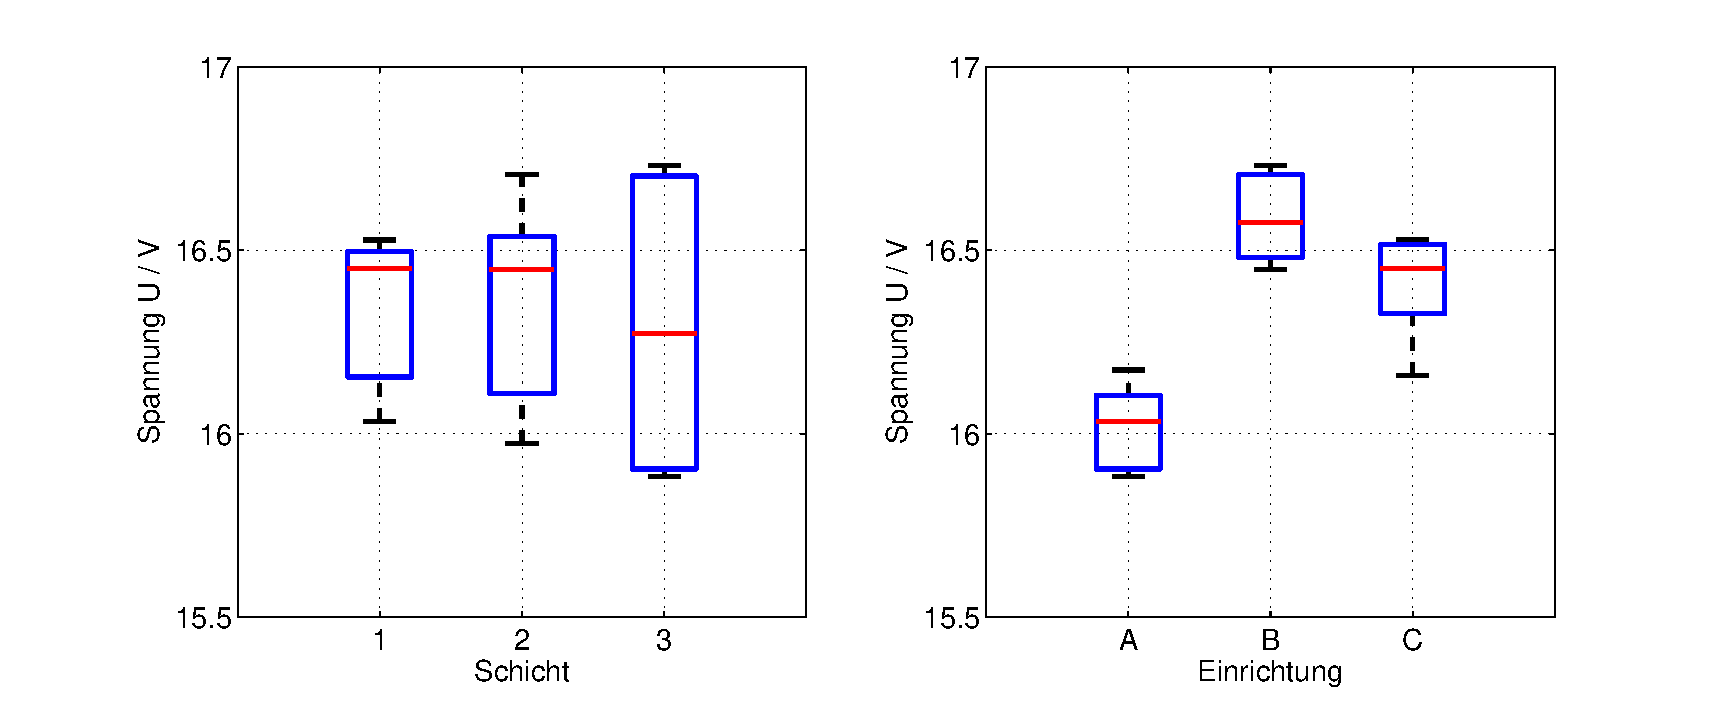
\includegraphics[width=1\textwidth]{Kapitel9/Bilder/image4}}
  \caption{Boxplot f\"{u}r die Vermessung von Spannungsreglern aus unterschiedlichen Abgleichstationen und unterschiedlichen Fertigungsschichten}
  \label{fig:VarianzanalyseZweifachSpannungsregler}
\end{figure}

\noindent An der \"{U}berlappung der Interquartil-Bereiche im linken Diagramm l\"{a}sst sich ablesen, dass die Schicht keinen signifikanten Einfluss auf das Abgleichergebnis hat. Der Box-Plot im rechten Diagramm best\"{a}tigt den signifikanten Einfluss der Einrichtung.

\clearpage 

\noindent Die Berechnung mit MATLAB ist in den folgenden Programmzeilen dargestellt.

\lstinputlisting[caption = {}]{Kapitel9/mat2.m}

\subsubsection{Varianzanalysen mit mehr als zwei Einflussgr\"{o}{\ss}en}

\noindent Varianzanalysen mit mehr Einflussgr\"{o}{\ss}en werden auf dieselbe Art durchgef\"{u}hrt, wie die ein- oder zweifaktorielle Varianzanalyse. Wegen des hohen numerischen Aufwands wird die Analyse typischerweise mit der Unterst\"{u}tzung eines Statistik-Programms durchgef\"{u}hrt, die jeweils unterschiedliche Syntax aufweisen. Gemeinsam ist die Darstellung des Ergebnisses als ANOVA-Tabelle, die die Zwischenergebnisse und das Ergebnis des Hypothesentests beinhaltet.

\subsubsection{ANOVA-Tabellen in MATLAB und Python}

\begin{table}[H]
\setlength{\arrayrulewidth}{.1em}
\caption{Varianzanalyse mit MATLAB}
\setlength{\fboxsep}{0pt}%
\colorbox{lightgray}{%
\arrayrulecolor{white}%
\begin{tabular}{ wc{8.3cm} | wc{8.3cm} }
\hline\xrowht{10pt}

\fontfamily{phv}\selectfont\textbf{MATLAB-Befehl} &
\fontfamily{phv}\selectfont\textbf{Funktionsbeschreibung} \\ \hline \xrowht{10pt}

\fontfamily{phv}\selectfont{anova1(\textbf{X})} & 
\fontfamily{phv}\selectfont{Einfaktorielle Varianzanalyse} \\ \hline\xrowht{10pt}

\fontfamily{phv}\selectfont{anova2(\textbf{X})} & 
\fontfamily{phv}\selectfont{Zweifaktorielle Varianzanalyse} \\ \hline\xrowht{10pt}

\fontfamily{phv}\selectfont{anova3(\textbf{X})} & 
\fontfamily{phv}\selectfont{N-Dimensionale Varianzanalyse} \\ \hline

\end{tabular}%
}
\label{tab:nineten}
\end{table}

\noindent In Python existieren unterschiedliche Methoden zur Berechnung einer Varianzanalyse. Eine universelle L\"{o}sung bietet die Bibliothek statsmodels.api, mit der auch Regressionsfunktionen berechnet werden k\"{o}nnen. Die Grundidee dabei ist, ein Modell kategorieller Variablen wie in Gleichung \eqref{eq:ninetwentyfive} zu definieren. Die konstante Gr\"{o}{\ss}e ist keine Varianzursache und wird deshalb nicht aufgef\"{u}hrt. Der zuf\"{a}llige Fehler wird implizit ber\"{u}cksichtigt und nicht explizit aufgef\"{u}hrt.

\begin{equation}\label{eq:ninesixtyone}
Modell=\alpha _{j} +\beta _{k} +\alpha \beta _{jk}
\end{equation}

\noindent F\"{u}r dieses Modell wird eine Varianzanalyse durchgef\"{u}hrt. Der folgende Programmausschnitt zeigt da Vorgehen f\"{u}r das Beispiel der Spannungsregeler aus Kapitel 9.2.3. 

\clearpage

\lstinputlisting[caption = {}]{Kapitel9/mat3.m}

\noindent Dabei sind die kategoriellen Variablen zum Beispiel als C(Linie) gekennzeichnet, das Produkt der kategoriellen Gr\"{o}{\ss}en wird als C(Linie):C(Schicht) implementiert. Der urspr\"{u}ngliche Datensatz sowie die entstehende ANOVA-Tabelle erwenden das Pandas Dataframe-Format. Das Dataframe-Format erlaubt au{\ss}erdem eine besonders elegante Darstellung der Boxplots zur Validierung des Ergebnisses.

\begin{table}[H]
\setlength{\arrayrulewidth}{.1em}
\caption{Varianzanalyse mit Python}
\setlength{\fboxsep}{0pt}%
\colorbox{lightgray}{%
\arrayrulecolor{white}%
\begin{tabular}{ wc{8.3cm} | wc{8.3cm} }
\hline\xrowht{10pt}

\fontfamily{phv}\selectfont\textbf{Python-Befehl} &
\fontfamily{phv}\selectfont\textbf{Funktionsbeschreibung} \\ \hline \xrowht{10pt}

\fontfamily{phv}\selectfont{statsmodels.formula.api.ols} & 
\fontfamily{phv}\selectfont{Definition der Modellgleichung} \\ \hline\xrowht{10pt}

\fontfamily{phv}\selectfont{statsmodels.api.stats.anova\_lm} & 
\fontfamily{phv}\selectfont{Duchf\"{u}hrung der ANOVA} \\  \hline

\end{tabular}%
}
\label{tab:nineeleven}
\end{table}

\clearpage

\subsection{Anwendungsbeispiel: Homogenit\"{a}tspr\"{u}fung eines Luftflusses}

\noindent Ein wesentliches Ziel des Umweltschutzes ist es, sch\"{a}dliche Emissionen m\"{o}glichst abzustellen oder so weit wie m\"{o}glich zu reduzieren, um die Umwelt vor Luft-, Boden- oder Gew\"{a}sserverschmutzung zu bewahren und Menschen vor Belastungen zu sch\"{u}tzen. In dem Bundes-Immissionsschutzgesetzt werden daher Grenzwerte f\"{u}r den Aussto{\ss} von Schadstoffen aus gro{\ss}en Feuerungsanlagen wie Kohlewerken definiert.\newline

\noindent Die Einhaltung dieser Grenzwerte muss in regelm\"{a}{\ss}igen Abst\"{a}nden durch zertifizierte \"{U}berwachungsstellen \"{u}berpr\"{u}ft werden. Um den Aufwand zu minimieren, ist es vorteilhaft, nur an einer Stelle im Abluftkanal messen zu m\"{u}ssen. Voraussetzung daf\"{u}r ist, dass die Emissionsverteilung \"{u}ber den Querschnitt des Abluftkanals ausreichend homogen ist. Der Homogenit\"{a}tstest entspricht einer einfaktoriellen Varianzanalyse. Das Abgas wird als homogen \"{u}ber den Querschnitt angesehen, wenn sich der Messwert zwar zeitlich \"{a}ndert, jedoch nicht von Messpunkt zu Messpunkt. Es wird deshalb \"{u}berpr\"{u}ft, ob die Abweichungen der Messwerte zuf\"{a}llig sind oder ob durch die Inhomogenit\"{a}t des Luftflusses der Gehalt der Messgr\"{o}{\ss}e in der Abluft variiert.

\noindent 
\begin{figure}[H]
  \centerline{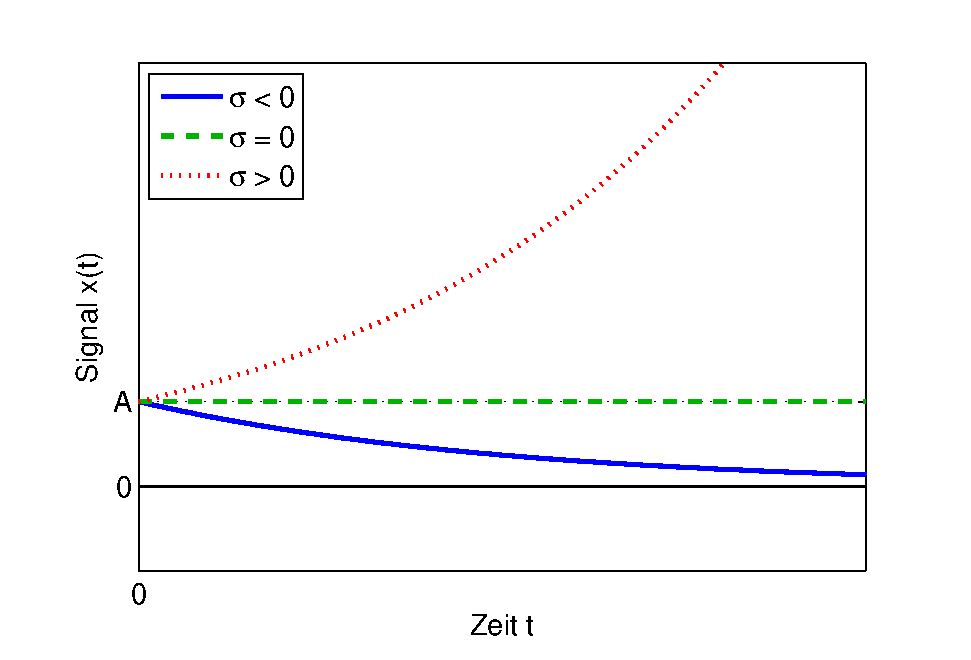
\includegraphics[width=0.8\textwidth]{Kapitel9/Bilder/image5}}
  \caption{Querschnitt durch den Abluftkanal mit unterschiedlichen Messachsen und Messpunkten}
  \label{fig:QuerschnittAbluftrohr}
\end{figure}

\noindent Liegt f\"{u}r die Anlage keine g\"{u}ltige Homogenit\"{a}tspr\"{u}fung vor, ist die Homogenit\"{a}t der Verteilung der Messgr\"{o}{\ss}e beziehungsweise eines Ersatzparameters im Messquerschnitt mithilfe von Netzmessungen und zus\"{a}tzlicher Vergleichsmessungen mit einer unabh\"{a}ngigen Messeinrichtung an einem festen Punkt innerhalb der Messstrecke zu ermitteln. Dabei werden an mehreren Stellen des Abluftkanals Messsonden eingebracht und bei unterschiedlicher Eindringtiefe der Messwert erfasst. Die Homogenit\"{a}tsbestimmung wird in diesem Beispiel f\"{u}r Stickoxide (NOx) durchgef\"{u}hrt. Hierzu wurden die in Tabelle \ref{tab:ninetwelve} aufgelisteten Messwerte aufgenommen. Parallel wird ein Referenzwert aufgenommen.

\clearpage

\begin{table}[H]
\setlength{\arrayrulewidth}{.1em}
\caption{Messreihe zur Homogenit\"{a}tsbestimmung f\"{u}r Stickoxide}
\setlength{\fboxsep}{0pt}%
\colorbox{lightgray}{%
\arrayrulecolor{white}%
\begin{tabular}{ wc{0cm} wc{3.3cm} | wc{4cm} | wc{4cm} | wc{4cm} }
\hline\xrowht{10pt}

&
\multicolumn{2}{c}{\fontfamily{phv}\selectfont{Messort}} &
\multirow{2}{*}{\fontfamily{phv}\selectfont{Netzmessung}} &
\multirow{2}{*}{\fontfamily{phv}\selectfont{Referenzmessung}}\\ \xrowht{10pt}

&
\fontfamily{phv}\selectfont{Messachse} & 
\fontfamily{phv}\selectfont{Messpunkt} &
&\\ \hline\xrowht{10pt}

&
\fontfamily{phv}\selectfont{1} & 
\fontfamily{phv}\selectfont{1} &
\fontfamily{phv}\selectfont{127} & 
\fontfamily{phv}\selectfont{125}\\ \hline\xrowht{10pt}

&
\fontfamily{phv}\selectfont{1} & 
\fontfamily{phv}\selectfont{2} &
\fontfamily{phv}\selectfont{132} & 
\fontfamily{phv}\selectfont{129}\\ \hline\xrowht{10pt}

&
\fontfamily{phv}\selectfont{1} & 
\fontfamily{phv}\selectfont{3} &
\fontfamily{phv}\selectfont{132} & 
\fontfamily{phv}\selectfont{131}\\ \hline\xrowht{10pt}

&
\fontfamily{phv}\selectfont{1} & 
\fontfamily{phv}\selectfont{4} &
\fontfamily{phv}\selectfont{109} & 
\fontfamily{phv}\selectfont{127}\\ \hline\xrowht{10pt}

&
\fontfamily{phv}\selectfont{2} & 
\fontfamily{phv}\selectfont{1} &
\fontfamily{phv}\selectfont{136} & 
\fontfamily{phv}\selectfont{126}\\ \hline\xrowht{10pt}

&
\fontfamily{phv}\selectfont{2} & 
\fontfamily{phv}\selectfont{2} &
\fontfamily{phv}\selectfont{148} & 
\fontfamily{phv}\selectfont{121}\\ \hline\xrowht{10pt}

&
\fontfamily{phv}\selectfont{2} & 
\fontfamily{phv}\selectfont{3} &
\fontfamily{phv}\selectfont{160} & 
\fontfamily{phv}\selectfont{118}\\ \hline\xrowht{10pt}

&
\fontfamily{phv}\selectfont{2} & 
\fontfamily{phv}\selectfont{4} &
\fontfamily{phv}\selectfont{152} & 
\fontfamily{phv}\selectfont{126}\\ \hline\xrowht{10pt}

&
\fontfamily{phv}\selectfont{3} & 
\fontfamily{phv}\selectfont{1} &
\fontfamily{phv}\selectfont{113} & 
\fontfamily{phv}\selectfont{107}\\ \hline\xrowht{10pt}

&
\fontfamily{phv}\selectfont{3} & 
\fontfamily{phv}\selectfont{2} &
\fontfamily{phv}\selectfont{132} & 
\fontfamily{phv}\selectfont{96}\\ \hline\xrowht{10pt}

&
\fontfamily{phv}\selectfont{3} & 
\fontfamily{phv}\selectfont{3} &
\fontfamily{phv}\selectfont{125} & 
\fontfamily{phv}\selectfont{101}\\ \hline\xrowht{10pt}

&
\fontfamily{phv}\selectfont{3} & 
\fontfamily{phv}\selectfont{4} &
\fontfamily{phv}\selectfont{125} & 
\fontfamily{phv}\selectfont{100}\\ \hline\xrowht{10pt}

&
\fontfamily{phv}\selectfont{4} & 
\fontfamily{phv}\selectfont{1} &
\fontfamily{phv}\selectfont{119} & 
\fontfamily{phv}\selectfont{98}\\ \hline\xrowht{10pt}

&
\fontfamily{phv}\selectfont{4} & 
\fontfamily{phv}\selectfont{2} &
\fontfamily{phv}\selectfont{127} & 
\fontfamily{phv}\selectfont{105}\\ \hline\xrowht{10pt}

&
\fontfamily{phv}\selectfont{4} & 
\fontfamily{phv}\selectfont{3} &
\fontfamily{phv}\selectfont{127} & 
\fontfamily{phv}\selectfont{105}\\ \hline\xrowht{10pt}

&
\fontfamily{phv}\selectfont{4} & 
\fontfamily{phv}\selectfont{4} &
\fontfamily{phv}\selectfont{134} & 
\fontfamily{phv}\selectfont{112}\\ \hline

\end{tabular}%
}
\label{tab:ninetwelve}
\end{table}

\noindent Netzmessung und Referenzmessung bilden eine Gruppe mit einem Stichprobenumfang von zwei Messungen. Die Differenz der Messwerte oder die Varianz innerhalb der Gruppe ist damit ein Ma{\ss} f\"{u}r die Genauigkeit der Messung selbst. \newline

\noindent Die Messungen werden an 16 Orten durchgef\"{u}hrt, sie bilden die Gruppen der Varianzanalyse. Die Varianz zwischen den Gruppen ist ein Ma{\ss} f\"{u}r die Homogenit\"{a}t des Abluftstroms.\newline

\noindent Bei einem homogenen Abluftstrom m\"{u}sste die Varianz von Messort zu Messort kleiner sein als die Varianz zwischen Netzmessung und Referenzmessung. Diese Annahme kann mit einer Varianzanalyse mit J = 16 Stichproben mit je einem Umfang von N = 2 Messwerten \"{u}berpr\"{u}ft werden. Die Auswertung ergibt die in Tabelle \ref{tab:ninethirteen} dargestellte ANOVA-Tabelle.

\clearpage

\begin{table}[H]
\setlength{\arrayrulewidth}{.1em}
\caption{Bewertung der Homogenit\"{a}t als ANOVA-Tabelle}
\setlength{\fboxsep}{0pt}%
\colorbox{lightgray}{%
\arrayrulecolor{white}%
\begin{tabular}{ wc{3.4cm} | wc{1.8cm} | wc{2.2cm} | wc{3.4cm} | wc{2cm} | wc{2cm} }
\hline\xrowht{10pt}

\fontfamily{phv}\selectfont{Streuungs-} &
\fontfamily{phv}\selectfont{Quadrat-} &
\fontfamily{phv}\selectfont{Freiheits-} &
\fontfamily{phv}\selectfont{Standardisierte} &
\fontfamily{phv}\selectfont{Wert der} &
\multirow{2}{*}{\fontfamily{phv}\selectfont{p-Wert}} \\ \xrowht{10pt}

\fontfamily{phv}\selectfont{quelle} &
\fontfamily{phv}\selectfont{summe} &
\fontfamily{phv}\selectfont{grade} &
\fontfamily{phv}\selectfont{Quadratsumme} &
\fontfamily{phv}\selectfont{Testvariable} &
\\\hline \xrowht{15pt}

\fontfamily{phv}\selectfont{Zwischen den Grup-} &
\multirow{3}{*}{\fontfamily{phv}\selectfont{3274.72}} &
\multirow{3}{*}{\fontfamily{phv}\selectfont{15}} &
\multirow{3}{*}{\fontfamily{phv}\selectfont{218.315}} &
\multirow{6}{*}{\fontfamily{phv}\selectfont{0.87}} &
\multirow{6}{*}{\fontfamily{phv}\selectfont{0.6043}} \\ \xrowht{15pt}

\fontfamily{phv}\selectfont{pen (Homogenität)} &
&
&
&
&
\\\cline{1-4} \xrowht{15pt}

\fontfamily{phv}\selectfont{Innerhalb der Grup-} &
\multirow{3}{*}{\fontfamily{phv}\selectfont{4016.5}} &
\multirow{3}{*}{\fontfamily{phv}\selectfont{16}} &
\multirow{3}{*}{\fontfamily{phv}\selectfont{251.031}} &
&
\\ \xrowht{15pt}

\fontfamily{phv}\selectfont{pen (Genauigkeit)} &
&
&
&
&
\\\hline \xrowht{15pt}

\fontfamily{phv}\selectfont{Gesamtstreuung} &
\fontfamily{phv}\selectfont{7291.22} &
\fontfamily{phv}\selectfont{31} &
&
&
\\ \hline

\end{tabular}%
}
\label{tab:ninethirteen}
\end{table}

\noindent Mit dem Signifikanzniveau $\alpha = 0.05$, den Freiheitsgraden $(J - 1)$ = 15 beziehungsweise $J\cdot (N - 1) = 16$ und der inversen F-Verteilung ergibt sich f\"{u}r 

\begin{equation}\label{eq:ninesixtytwo}
F(c)=1-\alpha =0.95
\end{equation}

\noindent die kritische Grenze c = 2.3522. Der Vergleich mit $v_{0}$ zeigt, dass $v_{0} < c $ ist. Die Hypothese, dass alle Mittelwerte gleich sind, wird deshalb best\"{a}tigt. Aufgrund der vorliegenden Stichprobe kann also angenommen werden, dass der Luftfluss homogen ist. Die Messwerte schwanken nur zuf\"{a}llig um den tats\"{a}chlichen NOx-Gehalt.\newline

\noindent Die Signifikanz des Messortes kann auch durch die Berechnung des p-Wertes gepr\"{u}ft werden. 

\begin{equation}\label{eq:ninesixtythree}
p=1-F\left(\dfrac{s_{\alpha }^{2} }{s_{\varepsilon }^{2} } \right)=60.43\%
\end{equation}

\noindent Da die Wahrscheinlichkeit p mit 60.43\% \"{u}ber dem gew\"{a}hlten Signifikanzniveau von $\alpha = 5\%$ liegt, kann die Nullhypothese nicht verworfen werden. Dies stimmt mit der Einsch\"{a}tzung aus dem Vergleich der Gr\"{o}{\ss}e $v_{0}$ mit der berechneten Grenze c \"{u}berein. Durch die Auswertung der Messwerte ist die Homogenit\"{a}t des Luftflusses nachgewiesen. Der Messpunkt kann somit frei gew\"{a}hlt werden. \newline

\noindent Die Auswertung der Messreihe wurde mit MATLAB durch die folgenden Programmzeilen durchgef\"{u}hrt.

\lstinputlisting[caption = {}]{Kapitel9/mat4.m}

\clearpage

\subsection{Literatur}

\begin{tabular}{|p{0.6in}|p{5.6in}|} \hline 
[Krey91] & Kreyszig, Erwin: Statistische Methoden und ihre Anwendungen\newline 4., unver\"{a}nderter Nachdruck der 7. Auflage\newline Vandenhoeck \& Ruprecht, G\"{o}ttingen, 1991 \\ \hline 
[Fahr96] & Fahrmeir, Ludwig; Hamerle, Alfred; Tutz, Gerhard: Multivariate statistische Verfahren\newline 2., \"{u}berarbeitete Auflage\newline Walter de Gryter \& Co., Berlin \\ \hline 
[Ross06] & Ross, M. Sheldon: Statistik f\"{u}r Ingenieure und Naturwissenschaftler\newline 3. Auflage\newline Spektrum Akademischer Verlag, M\"{u}nchen, 2006 \\ \hline 
[Hart07] & Hartung, Joachim; Elpelt, B\"{a}rbel: Multivariate Statistik\newline 7., unver\"{a}nderte Auflage\newline R. Oldenbourg Verlag, M\"{u}nchen / Wien \\ \hline 
[Papu01] & Papula, Lothar: Mathematik f\"{u}r Ingenieure und Naturwissenschaftler Band 3\newline 4., verbesserte Auflage\newline Vieweg Teubner, Braunschweig / Wiesbaden, 2008 \\ \hline 
\end{tabular}
